\begin{quote}
\textit{
``Where are you?'' Hiro says.
\\
\\
``In Reality or the Metaverse?''
\\
\\
``Both.''}
\end{quote}
\hfill \textit{Snow Crash, Neal Stephenson}
\\
\\
\\
Reviewing the literature on the domain of alternate realities this research finds that there is a gap in the scholarly investigation of simultaneous presence in real and virtual environments and the associated `vacancy problem'. This review proposes that a better understanding of the extension of human presence from only one of the real world or a virtual environment to simultaneous presence in both will permit the introduction of novel systems in a variety of fields in which simultaneous interaction and exploration of both real and virtual environments is possible. Such systems will likely be formed by expansion of research into \textit{cross reality}, an alternate reality comprised of complete real and virtual environments able to mutually reflect and influence each other via sensor/actuator infrastructure, and are likely to be in high demand as progress toward 3D extension of the Web continues.

\section{Introduction}
Research on alternate realities has been extensive, with the theme being explored for purposes as diverse as education~\cite{Warburton2009} and new forms of data visualisation~\cite{Coleman2009} to medical~\cite{TenEyck2011} and military training~\cite{Qiu2009}. Traditionally access to implementations of alternate realities was limited by the availability and high monetary cost of the specialised hardware and software that was required to create virtual environments and computerised superimpositions~\cite{Druck2006}. However more recently the cost and availability of this hardware and software has reduced and increased respectively to the point at which we find ourselves today where alternate realities can be, and in fact frequently are, experienced by many with the equipment they already have available to them with no special considerations~\cite{Sevan2008}.

Hardware capable of synthesising the graphically complex three-dimensional environments that alternate realities often present has reduced in cost to the point that it is no longer considered specialist equipment, owned only by those expressing an explicit interest in the subject, and is now commonplace in `average' consumer electronics devices, be they traditional desktop and laptop computers, games consoles, or portable devices such as mobile phones and tablets. Combined with the continued adoption of high-speed Internet connectivity~\cite{Cisco2011} the potential of multi-user virtual environments is already being realised, both for traditional competitive gaming through platforms such as World of Warcraft, but also for non-competitive purposes that focus more on community, creation and commerce with `virtual world' platforms such as Second Life~\cite{Sevan2008}.

Furthermore, progress toward ubiquity of sensing and actuating infrastructure in our everyday lives continues at an accelerated rate~\cite{Bose2009, Baronti2007}. Such systems are now commonplace in new buildings and also in consumer electronics, both portable devices such as mobile phones and tablets as well as home entertainment products such as games consoles. The result is that the amount of information that we can access about the physical and environmental state of a particular location at any given time is greater than ever.

The combination of these factors means that we are approaching the required dissemination of technology and public knowledge and understanding for virtual environments and integration with sensor/actuator infrastructure to begin making a larger impact on society and ultimately to be used by on a scale and in a manner similar to how the World Wide Web already is today. It is no longer preposterous to imagine a near future where a `Metaverse' reminiscent of that in Neal Stephenson's cyberpunk novel \textit{Snow Crash}, presenting an extension of the Web in the form of a three-dimensional virtual environment, has become a reality adopted by the majority of current Web users rather than remaining a vision of academics and cyberpunk fiction aficionados.

However although there are numerous examples of virtual environments, particularly those for competitive gaming, gaining substantial popularity~\cite{Sevan2008} and augmented reality and augmented virtuality products are no longer restrained to the research lab, this review has found very little research into simultaneous presence in \textit{complete} real and virtual environments. The term \textit{complete} is used to emphasise that the discussion here is about real and virtual environments that are both complete unto themselves and which can thus be explored and interacted with in isolation from the other, in addition to being explored simultaneously. This is a different concept to augmented reality and augmented virtuality systems, where the augmentations are usually near meaningless when separated from the context bestowed upon them by the underlying environment that they are augmented upon.

The \textit{cross reality} paradigm represents the most promising foray into investigation of this concept, as such a system is established through the combination of two complete environments, a real environment and a virtual environment that is based upon and mimics this real environment, which are bestowed with the abilities of mutual reflectance and influence through the use of sensor/actuator infrastructure (see section \ref{sec:cross_reality} for full discussion). Physical and environmental changes in the state of the real environment are captured by sensors and these data used to update the state of the virtual environment, whilst simultaneously changes in the state of the virtual environment manifest into the real environment via actuators. Users are free to explore and interact with either environment in relative isolation from the other, even if their interactions in one trigger changes in the other, however simultaneous interaction and exploration with both environments has largely remained without systematic investigation.

This is largely because users exploring and interacting with the real environment do not have a convenient manner of also exploring and directly interacting with the virtual environment, as such interaction usually relies upon the use of software run on a desktop or laptop computer which is not conducive to mobile use. Using a laptop computer whilst walking around is far from convenient and using a desktop computer obviously limits the user's interaction with the real environment to that immediately around the location of the  computer and results in a disjoint relationship between their physical position in the real environment and the location of their avatar in the virtual environment when they navigate their avatar away from the respective position of their computer. This situation has been called `the vacancy problem'; an apparent vacancy from one environment whilst engrossed in the other (see section \ref{subsec:dual_reality_:_an_emerging_medium} for full discussion).

Interested in the promise of simultaneous presence in complete real and virtual environments, particularly those that are able to mutually affect each other via sensor/actuator infrastructure and the cross reality paradigm, this literature review investigates how academic studies have treated such themes. The conclusion of this investigation is that the theme of simultaneous presence in real and virtual environments is still discussed only marginally in the scholarly literature and that this situation warrants attention as the benefits proposed by such interactions between real and virtual environments are extremely promising.

\section{Defining Alternate Realities}
A fundamental imperative for the remainder of this review is a well defined set of criteria for classifying and differentiating between different types of alternate reality. The terms \textit{mixed reality}, \textit{augmented reality} and to a lesser extent \textit{augmented virtuality} are all now relatively common in the literature, however they have too often been used in conflicting manners, or assigned vague definitions with uncertain boundaries separating them from each other. Furthermore the less well established terms \textit{cross reality} and \textit{X reality} (different names for the same concept) also need classifying according to the same system.

\subsection{Reality Continua}
Paul Milgram, Herman Colquhon and Fumio Kishino addressed this issue in detail and can in fact be accredited with introducing the terms \textit{augmented virtuality} and \textit{mixed reality} to the literature in the first instance, prompted by their identification of the need for more encompassing terms to supplement the existing definitions of \textit{augmented reality}~\cite{Milgram1994, Milgram1999}. Their discussion at times takes on a hint of the philosophical, as it rightly discusses what exactly it is that we mean by `real' and `virtual' and whether it is in fact reality or virtuality which is being augmented. However despite these thorough and well-reasoned definitions being published originally in 1994, much of the subsequent literature studied for this review has adopted conflicting, or at least confusing and misleading, definitions.

One of the overbearing concepts that Milgram et al. introduced is that whilst both purely real and purely virtual environments do exist they should not be considered discrete alternatives but rather poles lying at opposite ends of a linear scale called the \textit{Reality-Virtuality continuum}. The location of an environment along this continuum coincides with its location along a parallel \textit{Extent of World Knowledge continuum} where `world knowledge' refers to the amount of quantitative information that is associated with the content being presented, or in other words how much of the environment is being `modelled' by a computer. These continua are included as figure \ref{reality_virtuality_extent_of_world_knowledge_continuum}.

\begin{figure}[h]
\centering
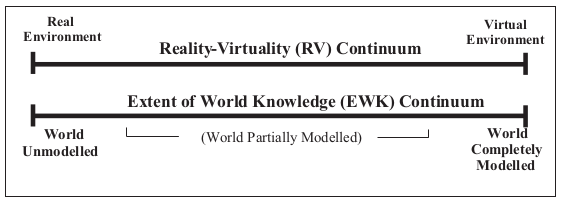
\includegraphics[width=0.8\textwidth]{reality_virtuality_extent_of_world_knowledge_continuum.png}
\caption{\textit{Reality-Virtuality continuum}, parallel with \textit{Extent of World Knowledge continuum}.}
\label{reality_virtuality_extent_of_world_knowledge_continuum}
\end{figure}

With a purely virtual environment, the entire viewport must necessarily be computer modelled in order to be rendered and as such there is complete quantitative information about all objects and between all objects being presented. At the opposite end of the spectrum with a completely real environment where none of the viewport is computer modelled there is no quantitative information associated with the content being displayed. At any point between the extremes the environment consists of a mixture of some modelled and some non-modelled content; with the computer associating quantitative information to, and between, the virtual objects, but not to the real objects or between the virtual and real objects.

Carrying the continuum concept further, Milgram et al. illustrate their understanding of the existing term \textit{augmented reality} and also introduce two related new terms; \textit{augmented virtuality} and \textit{mixed reality} (see figure \ref{reality_virtuality_mixed_reality_continuum.png}). In this fashion, \textit{mixed reality} is used to describe any environment that is not completely real or completely virtual; that is, it encompasses all positions on the continuum between the extremes. \textit{Augmented reality} is used to describe a real environment upon which virtual objects are overlain and \textit{augmented virtuality} is used to describe a virtual environment upon which objects sampled from the real world (such as video feeds) are overlain. It is also shown here that \textit{mixed reality} encompasses both \textit{augmented reality} and \textit{augmented virtuality}.

\begin{figure}[h]
\centering
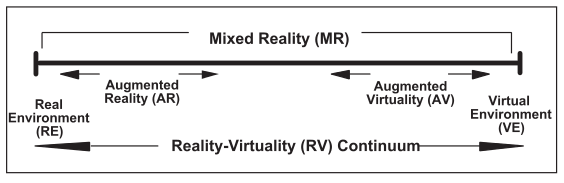
\includegraphics[width=0.8\textwidth]{reality_virtuality_mixed_reality_continuum.png}
\caption{Illustration of the terms \textit{mixed reality}, \textit{augmented reality} and \textit{augmented virtuality} within the context of the \textit{Reality-Virtuality} continuum.}
\label{reality_virtuality_mixed_reality_continuum.png}
\end{figure}

The obvious question raised from studying figure \ref{reality_virtuality_mixed_reality_continuum.png} is at what point toward the centre of the continuum an environment changes from being \textit{augmented reality} into \textit{augmented virtuality} or vice-versa. The answer lies with consideration of the quantitative knowledge associated with the objects that comprise the viewport.

For example, if one were to take a viewport depicting a purely real environment and then incrementally add more and more virtual objects, the environment's classification would progress rightward along the continuum. Eventually the entire viewport would be obscured by virtual objects and the obvious conclusion would be to classify the environment as being purely virtual. However this would only be true if there was complete quantitative information associated with, and between, all of the virtual objects within the real 3D space of the viewport, which is unlikely to be the case.

Likewise if one were to take a viewport depicting a purely virtual environment and incrementally replace the entire viewport with sampled real objects we could not classify the resultant environment as purely real as there would be associated quantitative knowledge with and between the sampled objects, meaning that the environment isn't completely unmodelled and thus can't be classified as purely real.


Thus, Milgram et al. conclude, it is not necessarily true that an environment is purely virtual simply because all of the visible objects are computer modelled, nor is it necessarily true that an environment is purely real simply because all of the visible objects are sampled from the real world.

\subsection{Reality Matrix}
\label{subsec:reality_matrix}
Another useful method of illustrating the relationships between the different categories of alternate realities was put forward by Roy Want in his introductory article for a 2009 issue of IEEE Pervasive Computing dedicated to the \textit{cross reality} paradigm~\cite{Want2009}. Here he presented a 2x2 matrix categorising the different terms according to whether the experience and overlay data are real or virtual (see figure \ref{original_virtuality_matrix.png}).

\begin{figure}[h]
\centering
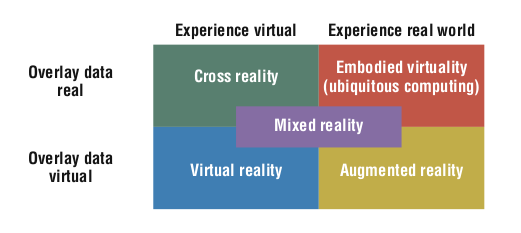
\includegraphics[width=0.8\textwidth]{original_virtuality_matrix.png}
\caption{Want's original virtuality matrix.}
\label{original_virtuality_matrix.png}
\end{figure}

Whilst this is a useful representation, some of the definitions and criteria depicted do not match with those of Milgram et al. or even with those of other authors in the same issue of IEEE Pervasive Computing, let alone other publications concerning alternate realities. Thus this review presents a modified version of Want's matrix, that is better in fitting with the consensual definitions built from reviewing the literature on alternate realities, as figure \ref{modified_virtuality_matrix.png}.

\begin{figure}[h]
\centering
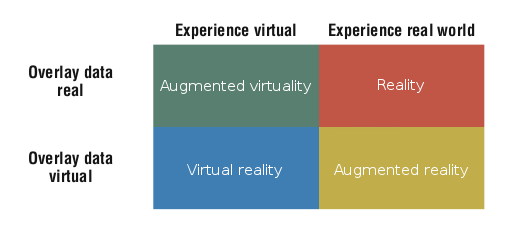
\includegraphics[width=0.8\textwidth]{modified_virtuality_matrix.png}
\caption{Want's virtuality matrix after modification by this review; note removal of \textit{mixed reality}, \textit{cross reality} and \textit{embodied virtuality} and addition of \textit{reality} and \textit{augmented virtuality}.}
\label{modified_virtuality_matrix.png}
\end{figure}

Where Want has \textit{cross reality} occupying the upper left quadrant at the congruence of `experience virtual' and `overlay data real' this review instead places \textit{augmented virtuality}. Referring to Milgram's continuum `experience virtual' relates to a position somewhere on the right half, while `overlay data real' relates to presentation over this virtual environment of sampled real world data resulting in a partially modelled environment, leaving us in the area of the continuum occupied by \textit{augmented virtuality}.

Want's matrix also features the term \textit{embodied virtuality} in the upper right quadrant, at the congruence of `experience real world' and `overlay data real'. Want explains that this is an alternative term for \textit{ubiquitous computing} which is \textit{``essentially the opposite of VR''}; this review instead reasons that the opposite of \textit{virtual reality} is simply \textit{reality} and that \textit{ubiquitous computing} does not constitute an alternate reality but simply a different model of human-computer interaction that can be implemented in either \textit{reality} or \textit{augmented reality}, depending upon how the computing infrastructure presents information to users.

A \textit{ubiquitous computing} system is necessarily a real environment, as it is by definition the integration and dissemination of computational infrastructure into our real surrounds~\cite{York2004}. However whether this real environment is augmented by virtual objects is not restricted by the concept. Thus \textit{ubiquitous computing} can exist in an environment that is either on the left extreme of the continuum, where no virtual objects are employed and the environment remains completely unmodelled, or somewhere to the right of the left extreme in the region of \textit{augmented reality}, where virtual objects are employed and the environment is partially modelled.

This line of reasoning is supported by an almost complete lack of further mention of \textit{ubiquitous computing} elsewhere in the literature about alternate realities studied for this review. Furthermore the term \textit{embodied virtuality} is not used by any other author in the studied literature.

Finally this review has removed the central \textit{mixed reality} section from Want's original matrix, as its position could be misleading. As the boundaries formed between the categories by the different colours could be construed as meaning that there are discrete boundaries between the different categories, rather than a linear scale as depicted by Milgram's continuum, the reader could be led to believe that a purely \textit{virtual reality} or a purely \textit{embodied virtuality} environment can be considered \textit{mixed reality}, which is incorrect. If one wishes to picture the position of \textit{mixed reality} in relation to the modified matrix, it would cover the same area as enclosed by the union of \textit{augmented virtuality} and \textit{augmented reality}.

\subsection{More Reality Continua}
As one of the most prominent academics in the development of the cross reality paradigm (see section \ref{sec:cross_reality}) it is also worth comparing Joshua Lifton's definitions for the different categories of alternate realities and the relationships between them~\cite{Lifton2007a} in the current context.

Lifton's definitions, or more accurately his relationships between, the terms \textit{reality}, \textit{augmented reality}, \textit{mixed reality} and \textit{virtual reality} do not perfectly match the consensus that this review has observed. Lifton defines the terms individually in agreement with the consensus, however doesn't proffer the conclusion that mixed reality is a broad term that includes augmented reality. He also doesn't mention augmented virtuality, even though the Dual Reality Lab project (see section \ref{subsec:mit_shadow_lab}) does implement it. Finally his diagram that alludes to Milgram's continua and is included as figure \ref{original_lifton_axis.png}, situates mixed reality at an incorrect position, implying that Lifton's definition of mixed reality is of a discrete state to that of augmented reality, even though his textual definition of mixed reality hints that it logically encompasses augmented reality. This review presents a modified version of Lifton's diagram to illustrate these differences as figure \ref{modified_lifton_axis.png}.

Lifton does however explain that while such a taxonomy can be successfully applied to most alternate reality efforts, it does not well address the concept of cross reality where there are two complete realities, one real and one virtual.

\begin{figure}[h]
\centering
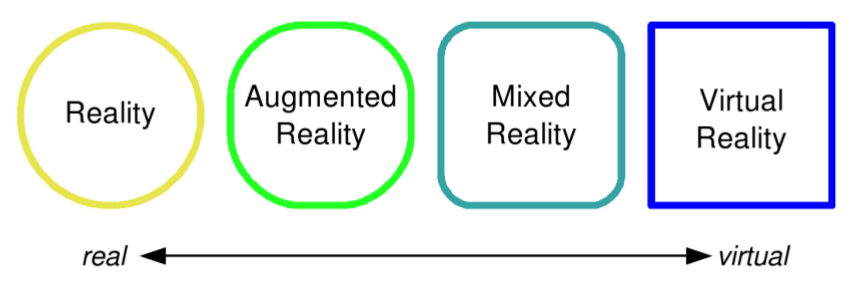
\includegraphics[width=\textwidth]{original_lifton_axis.png}
\caption{The \textit{``virtual worlds taxonomy as viewed on the real-virtual axis''} presented by Lifton.}
\label{original_lifton_axis.png}
\end{figure}

\begin{figure}[h]
\centering
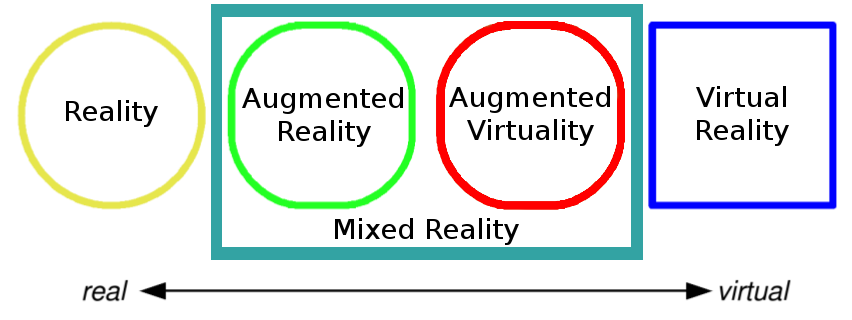
\includegraphics[width=\textwidth]{modified_lifton_axis.png}
\caption{Lifton's taxonomy as modified by this review.}
\label{modified_lifton_axis.png}
\end{figure}

\section{Adopted Definitions of Alternate Realities}
\label{sec:definitions_of_alternate_realities}
This review has discovered differing (and in some cases conflicting) definitions for the different categories of alternate realities and for the criteria for differentiating between them. What follows in this section represents the definitions and differentiating criteria that this review has adopted after concluding them the most widely accepted and well reasoned.

\subsection{Reality}
Occupying the left extreme of Milgram's continuum and the upper right quadrant of the modified Want matrix, \textit{reality} refers to an environment that is entirely unmodelled, with the viewport containing no virtual objects and no computer-based quantitative information is associated with any of the (necessarily real) objects. In fact, there may be no computer infrastructure involved in the situation whatsoever. This is the situation that we are most familiar with, as it is where the vast majority of us spend the vast majority of our time.

\subsection{Virtual Reality}
The polar opposite to \textit{reality}, a \textit{virtual reality} environment occupies the right extreme of Milgram's continuum and the lower left quadrant of the modified Want matrix. A \textit{virtual reality} environment consists solely of virtual objects, with computer-based quantitative information associated with all of them and between all of them, creating a completely synthetic world entirely discrete and separate from the real world; a new world that exists solely within the data structures of a computer.%cite Milgram and Want

Traditional definitions of \textit{virtual reality} require the environment to be completely immersing; that is, when involved with such an environment the user is completely unaware of the real environment that surrounds their real bodies, often making use of Head Mounted Displays (HMD) and head \&/or body tracking techniques to improve the sense of immersion by removing the need to interact with interfaces logically anchored to the real world such as keyboards, mice and joysticks~\cite{Druck2006}.

However this review believes that taking the concept to a lesser extreme, the virtual environments presented by video games such as World of Warcraft can be construed as \textit{rudimentary} implementations of virtual reality; they are completely modelled environments that exist entirely separate to the real world, however interaction is not completely immersing due to the use of 2D monitors and traditional interface devices, largely due to the lack of common ownership of HMDs and advanced body tracking systems.

\subsection{Mixed Reality}
Occupying any position between the extremes on Milgram's continuum, the term \textit{mixed reality} refers to a broad range of environments that arise from the merging of real and virtual environments to some extent such that the result is neither entirely real nor entirely synthetic, where real and virtual objects co-exist. As alluded to previously, under this definition both \textit{augmented reality} and \textit{augmented virtuality} are included under the broader classification of \textit{mixed reality}.

This is one definition where Want is lacking, claiming \textit{mixed reality} to be \textit{``some combination of the others''} where `others' refers to all of \textit{virtual reality}, \textit{augmented reality}, \textit{embodied virtuality} and \textit{cross reality}. This review disregards this definition as it relies upon Want's previously refuted definition of \textit{embodied virtuality} being the polar opposite of \textit{virtual reality} and because it also depends upon Want's definition of \textit{cross reality} which this review will also go on to refute.

\subsection{Augmented Reality}
An \textit{augmented reality} environment occupies a position within the `left half' of Milgram's continuum, the lower right quadrant of the modified Want matrix and within the broader classification of \textit{mixed reality}. Thus an \textit{augmented reality} environment comprises a real environment that has had virtual objects added to or overlain upon it; a common approach for achieving this addition/overlay is superimposing virtual objects over a direct or indirect view of the real environment using Head Mounted Displays \&/or cameras~\cite{Krevelen2010}.

A commercial example of \textit{augmented reality} is the Layar browser for mobile phones, which overlays various forms of data onto the view captured by a phone's camera after determining its location and orientation using GPS, accelerometer and magnetometer readings~\cite{eishita:layar}

%~\cite{Milgram1999}

\subsection{Augmented Virtuality}
Logically opposite to \textit{augmented reality}, an \textit{augmented virtuality} environment occupies a position within the `right half' of Milgram's continuum, the upper left quadrant of the modified Want matrix and again lies within the broader classification of \textit{mixed reality}. Thus an \textit{augmented virtuality} environment comprises a virtual environment, akin to \textit{virtual reality}, upon which sampled real objects are overlain, perhaps through the use of cameras~\cite{caballero:behand}.

A simple commercial example of augmented virtuality is the EyeToy accessory and associated software for Sony's Playstation 2 games console (and later the Playstation Eye for the Playstation 3), a digital camera that captures images of players and their surroundings and integrates them into the gaming experience presented on the screen.

\section{Cross Reality}
\label{sec:cross_reality}
The discussion of the literature pertaining to the \textit{cross reality} paradigm warrants its own section of this review, as it is not only one of the youngest categories included under the umbrella term \textit{alternate reality} but also the closest existing concept to lend to the simultaneous exploration of real and virtual environments.

First a brief overview of the paradigm is presented, that represents the conclusions drawn after studying the available literature on the subject. This is followed by an in-depth study of the literature that led to these conclusions, arranged largely chronologically to show what parties were responsible for the paradigm's creation and development from its inception.

As cross reality is a relatively recent concept that hasn't received a vast amount of scholarly attention, this section of the review represents an almost exhaustive survey of the literature published on the subject. For such a recent concept that is still open to debate and investigation, it is prudent to discuss all of the work that has thus far contributed to the field in any manner, rather than trying to judge contributions at such an early stage when the bounds of the subject matter are not yet well established or agreed.

\subsection{Overview of Cross Reality}
Cross reality is the ubiquitous mixed reality situation that arises from the fusion of real-world sensor/actuator infrastructure with virtual environments, such that augmented reality and augmented virtuality manifest simultaneously and facilitate synchronous multi-directional exchange of media and control information between real and virtual environments. Sensors collect and tunnel dense real-world data into virtual environments where they are interpreted and displayed to dispersed users, whilst interaction of virtual participants simultaneously incarnates into the real world through a plenitude of diverse displays and actuators~\cite{Paradiso2009}.

The principle features that distinguish cross reality from other alternate realities that this review has thus far covered are;
\begin{enumerate}
	\item a shift from single- to bi-directional information flow between real and virtual environments~\cite{kim:practical}
	\item that both environments are complete unto themselves (but are enriched by their ability to mutually reflect, influence and merge into one another).~\cite{lifton:merging}
\end{enumerate}

Because a cross reality system is comprised of two complete environments, it cannot be placed at a single point on Milgram's continuum but instead occupies two separate points, one to the left and the other to the right of the centre. Similarly with the modified Want matrix, a cross reality system would occupy one location in the upper left quadrant of augmented virtuality and a second in the lower right quadrant of augmented reality. 

\subsection{MIT Media Lab Responsive Environments Group}
\label{subsec:responsive_environments_at_mit_media_lab}
The Responsive Environments Group at MIT's Media Lab, under the direction of Joseph Paradiso, deserve the accolade for the inaugural work in establishing cross reality as a field of research. In their own words, the group \textit{``explores how sensor networks augment and mediate human experience, interaction and perception''}~\cite{ResponsiveEnvironmentsGroup} and since 1995 they have produced prolific research in the domain of sensor architecture and wireless sensor clusters~\cite{Paradiso1996, Rowe1999, Burke1996, Paradiso1997, Knaian2000, Teegarden2001, A2007, Ma2002, Bamberg2008, Laibowitz2005, LaPenta2007} and perceptive spaces~\cite{Lifton2001, Paradiso1997a, Paradiso2000, Richardson2004}, establishing a prime research environment, both in terms of experience and available technologies, for a concept such as cross reality to emerge.

The path to cross reality began with the `Plug' project that created a sensor network comprising power strips imbued with sensing, computational and communicative abilities~\cite{Lifton2007b}. By basing the nodes on power strips the platform was ideally suited for broad and unobtrusive deployment in environments where people work and live as power strips already exist in such environments with ubiquity. A labelled photograph of a single Plug node is included as figure \ref{mit_plug.jpg}. In addition to sporting a number of different sensors, each Plug node was also able to individually control the output of the four 120Vac sockets, allowing the nodes to act as both input (sensing) and output (actuating) devices.

\begin{figure}[h]
\centering
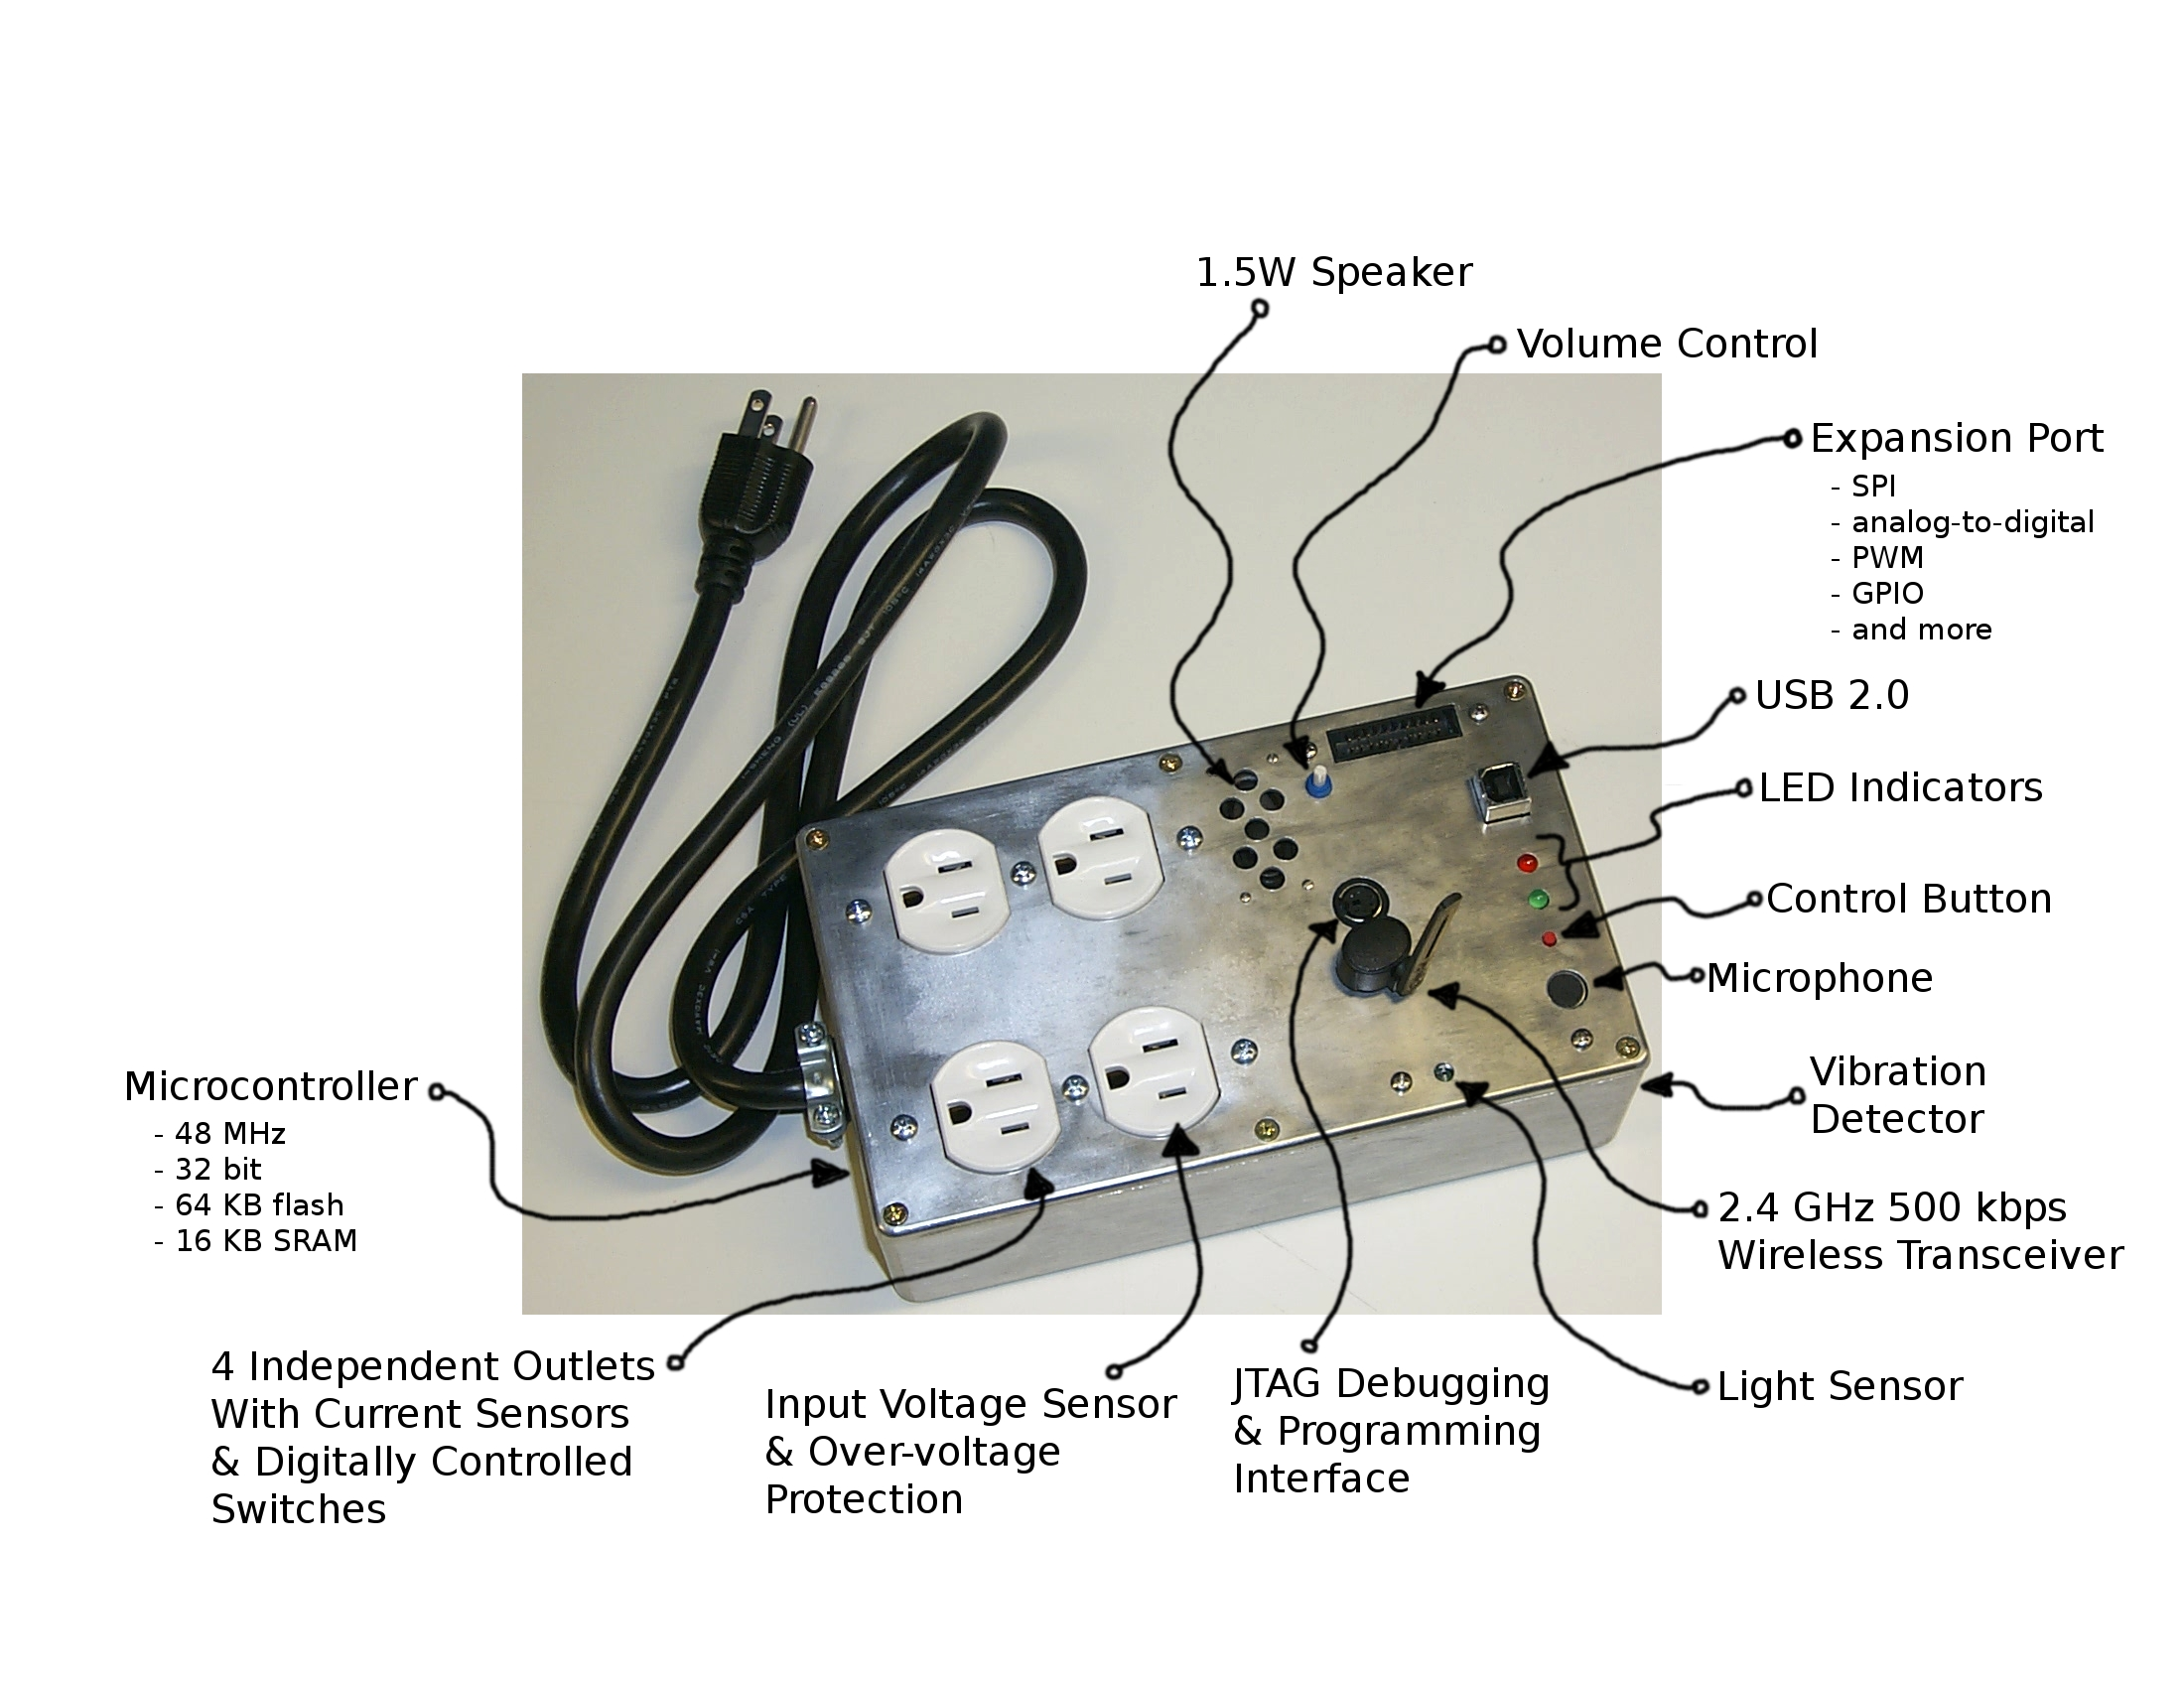
\includegraphics[width=\textwidth]{mit_plug.jpg}
\caption{A Plug node.}
\label{mit_plug.jpg}
\end{figure}

Parallel to the development of the Plug platform the group also developed two mobile platforms for interacting with the network of nodes. The Tricorder project~\cite{Lifton2007}, based around a Nokia 770 Internet tablet, presented users with a two-dimensional map centered and oriented about the Tricorder's physical position and allowed \textit{``real-time point-and-browse''} functionality to browse the sensor data from nodes within the vicinity. The Ubicorder~\cite{Mittal2011} project made use of a tablet laptop computer and allowed users to graphically define, and recursively combine, rules for translating sensor data to higher order and potentially more meaningful events.

The true birth of cross reality at the Media Lab came from the combination of the Plug platform with the Second Life virtual world in the Dual Reality Lab project which is comprehensively covered in Joshua Lifton's PhD thesis entitled `Dual Reality: An Emerging Medium'~\cite{Lifton2007a} and summarized in~\cite{lifton:merging}. The term `dual reality' would later evolve into what we now know as `cross reality', an association confirmed by Lifton himself~\cite{lifton:adoption}. As the inaugural work in establishing the field and framing cross reality as a new application domain for sensor/actuator infrastructure, virtual environments and media creation, and still by far the most exhaustive discussion of the paradigm, Lifton's thesis deserves closer attention in this reivew than other publications.

\subsection{Dual Reality: An Emerging Medium}
\label{subsec:dual_reality_:_an_emerging_medium}
In his 2007 thesis Lifton defines dual reality as
\begin{quote}
\textit{``An environment resulting from the interplay between the real world and the virtual world, as mediated by networks of sensors and actuators. While both worlds are complete unto themselves, they are also enriched by their ability to mutually reflect, influence, and merge into one another.''}~\cite{Lifton2007a}
\end{quote}
The key points to identify in this definition, which are confirmed later in the thesis and by other authors in subsequent literature, are that data flow is bi-directional between real and virtual environments and that the two environments are complete unto themselves in addition to having the ability to affect each other.

Perhaps the most interesting and topical discussion within Lifton's thesis for the purposes of this literature review, whose topic is simultaneous presence in complete real and virtual environments, is the discussion of what he calls \textit{`the vacancy problem'}, which he defines as
\begin{quote}
\textit{``the noticeable and profound absence of a person from one world, either real or virtual, while they are participating in the other. Simply put, the vacancy problem arises because people do not currently have the means to be in more than one place (reality) at a time. In the real world, the vacancy problem takes the form of people appearing completely absorbed in their virtual reality, to the exclusion of everything in the real world. In the virtual world, the vacancy problem takes the form of virtual metropolises appearing nearly empty because there are not enough avatars to fill them.''}
\end{quote}
Lifton identifies that this vacancy problem is a fundamental characteristic of the current generation of virtual worlds and proposes dual reality, more closely linking the real world with the virtual world, as an approach to mitigate the problem.

Lifton also surveys a range of interesting previous work broadly related to the concept of coupling the real world with virtual worlds. He roughly categorises these into those that attempted to bring a virtual world into the real world (augmented reality) and those that attempted to bring the real world into a virtual world (augmented virtuality). However upon further investigation one of the projects Lifton mentions, from IBM UK, reveals experiments with two way control mechanisms between real and virtual worlds which alludes more directly to the cross reality paradigm.

\subsection{IBM Virtual Universe Community}
IBM was influential in the 2006-2009 wave of virtual worlds,their involvement starting through grass roots interests on internal blogs and on Second Life~\cite{Hughes2006, Hughes2006a,Hughes2006b} from people such as Ian Hughes, at the time an IBM Software Strategist, and eventually expanding to include around 8000 employees (including the CEO at the time) and the creation of an Emerging Business Unit (EBO) - IBM's way to venture capital new ideas and see how they fit. A number of impressive projects were undertaken, the most high profile of which were the Wimbledon projects of 2006, 2007 and 2008~\cite{Hughes2006c, Hughes2009}. Journalist Rita King provided a good write-up of the entire story of the `Virtual Universe Community' at IBM~\cite{King2008} and various projects were featured by both Businessweek~\cite{Life2006} and the BBC~\cite{Mason2007}.

Ian Hughes confirmed via email to this review the extent toward a cross reality system that these investigations progressed

\begin{quote}
\textit{``The control mechanisms worked two ways generally. There was a physical lab that had devices that were controlled by a pub/sub mechanism based on the light weight protocol MQTT. Those devices subscribed to various messages. So initially web pages controlled them. The web page generated the message that was broadcast to everything that was interested, sending on/off messages. Equally the objects generated messages when they were physically switched on and off. As SL had an RPC interface it was possible (using another software component outside of SL) to subscribe to the same messages and send requests into SL to change states of object. Likewise it was simple to make an object when clicked or some other event in SL send a message back out. So there were lights, blinds, proximity detectors and even the tilt sensors on the laptops that were instrumented with these messages.''}
\end{quote}

So whilst Lifton and the other researchers at the Media Lab cannot necessarily be credited with `inventing' cross reality or performing the very first implementation of it, they deserve the accolade for being the first to perform an in-depth academic investigation into the concept, framing it as a new area of research interest.

\subsection{Shadow Lab}
\label{subsec:mit_shadow_lab}
The most impressive creation of the MIT Dual Reality Lab project was the `Shadow Lab', \textit{``a space in Second Life modelled after the third floor of the MIT Media Lab's Wiesner building, where the Plug sensor network is most often deployed''}. This comprised a to-scale two-dimensional floor plan of the entire third floor of the building and a three-dimensional reconstruction of the Media Lab itself.

Around the Shadow Lab were distributed a number of `data ponds' that each represented the data from a single Plug node. Each pond consisted of a number of waving stalks growing out of a puddle of water on the ground, with the different types of data affecting the appearance of different features; light affecting the pattern of the stalks' skin, temperature affecting their colour, motion affecting the stalks' motion, sound affecting the size of the puddle and electrical current (of devices drawing power from the 120Vac sockets of the Plug node) affecting the intensity of ethereal foxfire rising from amongst the stalks. These virtual data ponds allowed for the real-to-virtual, augmented virtuality aspect of the system. Inversely real world versions of the data ponds, each comprising a desk fan shrouded with lightweight plastic, allowed for the virtual-to-real, augmented reality aspect of the system. The airflow through the shroud, and thus the height and sound produced, could be controlled by pulse width modulating the output of the 120Vac sockets of the Plug nodes. Figure \ref{lifton_data_ponds.png} shows a virtual data pond (at left) and a number of real data ponds (at right) and figure \ref{lifton_shadow_lab.png} shows the final Shadow Lab itself.

\begin{figure}[h]
\centering
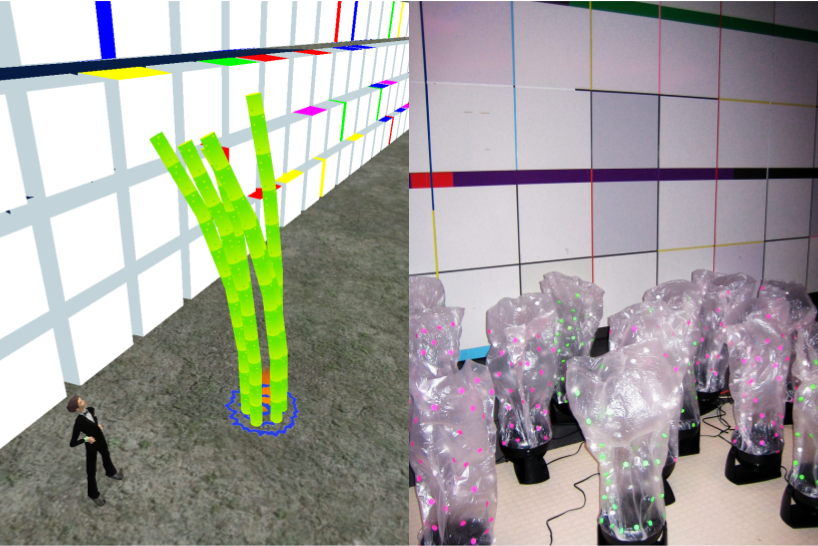
\includegraphics[width=\textwidth]{lifton_data_ponds.png}
\caption{Virtual (left) and real (right) data ponds.}
\label{lifton_data_ponds.png}
\end{figure}

\begin{figure}[h]
\centering
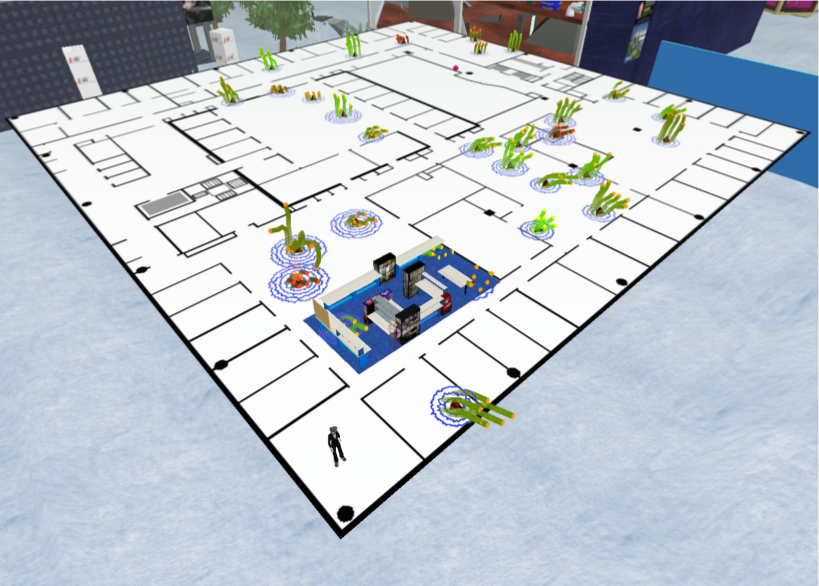
\includegraphics[width=\textwidth]{lifton_shadow_lab.png}
\caption{Side view of the final Shadow Lab structure, showing the two-dimensional floor plan of the third floor of the Wiesner building, three-dimensional reconstruction of the Media Lab, virtual data ponds and a human-sized avatar.}
\label{lifton_shadow_lab.png}
\end{figure}

Lifton evaluates the Dual Reality Lab project and makes the prudent observation that widespread adoption of the cross reality paradigm will rely upon sensor/actuator infrastructure as pervasive as today's electrical and lighting systems and online virtual worlds as populated as today's World Wide Web, both of which are years if not decades away. He also notes that even if these technologies do come to pass, the emergence of cross reality is not certain.

\subsection{Ubiquitous Sensor Portals}
Following on from the Dual Reality Lab, and now dropping the title dual reality in favour of cross reality, the Ubiquitous Sensor Portal project situated 45 I/O rich `portals', shown in figure \ref{ubiquitous_sensor_portal.jpg}, throughout the Media Lab, each with a corresponding extension in Second Life. Each portal comprised a myriad of environmental sensors (passive infrared (PIR) motion, light, sound, vibration, temperature and humidity) in addition to multimedia abilities via a camera, mounted on a motorised pan/tilt platform and capable of capturing still images as well as DVD-quality video, microphone and small touch screen display. They also featured active IR links that allowed them to communicate with various wearable badges in development by Media Lab researchers to identify users stood at a portal, and in addition could be used as reflection proximity sensors to detect the presence of unbadged users. When a user is present at a real portal, a white `ghost' is displayed by the corresponding virtual portal if they cannot be identified by badge, and their name displayed if they can. Video and audio from the real portal can be streamed into Second Life and a stream from a Second Life client streamed to the screen of the real portal.

\begin{figure}[h]
\centering
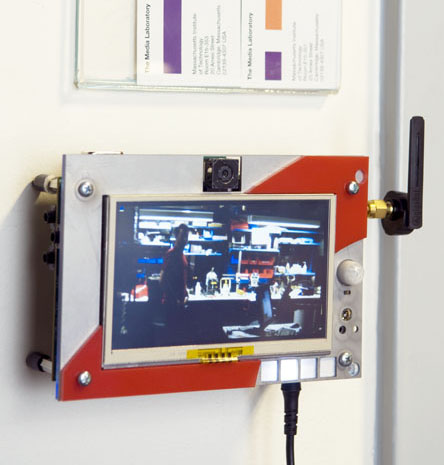
\includegraphics[width=0.6\textwidth]{ubiquitous_sensor_portal.jpg}
\caption{A Ubiquitous Sensor Portal.}
\label{ubiquitous_sensor_portal.jpg}
\end{figure}

However in stark contrast to the Dual Reality Lab, the virtual portals were not situated in a simulation of the real Media Lab in situations corresponding to their physical location, but instead used a more abstract virtual representation with a geometric layout; this design, shown in figure \ref{ubiquitous_sensor_portal_virtual.png}, reflected intellectual affiliation as opposed to real-world location and also allowed for intuitive browsing of past still images and videos captured by the real portal.

\begin{figure}[h]
\centering
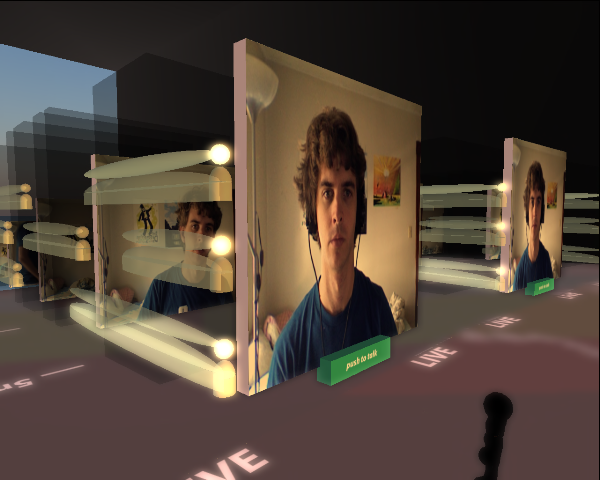
\includegraphics[width=0.8\textwidth]{ubiquitous_sensor_portal_virtual.png}
\caption{The design of the virtual portals in the Ubiquitous Sensor Portals project.}
\label{ubiquitous_sensor_portal_virtual.png}
\end{figure}

The ability of a person to walk about the real building and for their presence in front of different portals to be reflected in Second Life addressed the vacancy problem to some extent by allowing the user to explore the real environment in a normal fashion but for their position to occasionally be updated in the virtual environment. However the abstract layout of the virtual environment presents a method of virtual environments exploration disjoint to the physical layout and relationship between the portals themselves, which is not ideal for all applications.

\subsection{Doppellab}
\label{subsec:doppellab}
The current cross reality project undertaken by the Media Lab is the ongoing Doppellab, \textit{``an immersive, cross-reality virtual environment that serves as an active repository of the multimodal sensor data produced by a building and its' inhabitants''}~\cite{Dublon2011, Dublon2011a}. Doppellab uses the Unity3d game engine to allow users to visualise current and historic sensor data captured by a wide range of sensors distributed throughout the Media Lab in a three-dimensional virtual reconstruction.

However despite claiming to be a cross realtiy project, there is no evidence in the associated literature of any virtual-to-real, augmented virtuality data flow, which is a requirement of a cross reality system. Furthermore with regards to the vacancy problem, Doppellab \textit{``focuses on encouraging and enriching individual users' experiences of sensor data in 3-d environments''} and as such is of only passing interest to this review, as simultaneous presence in real and virtual environments must inherently support multiple users present in the same real and virtual surroundings to be of any great use.

\subsection{Consumer Adoption of Cross Reality}
\label{subsec:consumer_adoption_of_cross_reality}
A final piece of literature to consider whilst reviewing MIT's involvement with the cross reality paradigm and the vacancy problem, is an article written by Joshua Lifton, as an invited paper for the International Symposium on Ubiquitous Virtual Reality 2010, entitled \textit{Consumer Adoption of Cross Reality}. This is a retrospective piece, written after Lifton had left MIT in 2007 to work at the Electric Sheep Company, \textit{``then the premier third-party services company for designing, building and managing experiences across a number of virtual worlds, with a focus on Second Life''}, and in 2009 leaving the Electric Sheep Company to become an independent contractor and consultant. Lifton reasons that \textit{``these experiences and the transition from academia to industry helped shape my views on what is possible and what is probable in the field of cross reality''}.

The overall conclusion of the paper is that cross reality hadn't yet achieved notable consumer adoption because the full utility of ubiquitous computing, particularly in terms of sensing and actuating infrastructure, and virtual worlds had yet to be realised as they hadn't been fully developed and deployed. As the key enabling technologies of cross reality, their full realisation is required before the paradigm can begin to be widely adopted.

As discussed in further detail in section \ref{subsec:virtual_environments}, virtual worlds, particularly Second Life, failed to live up to their media hype, however the adoption and integration of sensor/actuator infrastructure into consumers' everyday lives has faired much better. Mobile phones with myriad sensors are now commonplace, on-body and off-body motion sensing have been extremely popular for games consoles (Nintendo Wii and Microsoft Kinect respectively), non-contact identification (RFID) is common in passports and building access and new buildings are now more often than not equipped with various sensing \&/or actuating capabilities in the form of Building Automation Systems (BAS).

\subsection{X-Reality}
\label{subsec:x-reality}
Marie Kim, Hwang Jae Gak and Cheol Sig Pyo at The Electronics and Telecommunications Research Institute, Korea, produced a Universal Sensor Network (USN) middleware, COSMOS, to address the issue of heterogeneity of sensor/actuator infrastructure that leads to difficulty in integrating them with virtual environments to establish a cross reality, or as they write it `X-reality', system~\cite{kim:practical}.

The matter of standards with relation to cross reality is discussed further in section \ref{subsec:sensor_actuator_infrastructure} however Kim et al.'s article is mentioned here as its introduction section frames and explains the cross reality paradigm well in terms of the principle features

\begin{quote}
\textit{``The important point of X-reality is a paradigm shift from single-directional information flows to bidirectional information flows between two worlds.''}
\end{quote}

and also how it can be employed for simultaneous presence in real and virtual environments

\begin{quote}
\textit{``The differential characteristic of X-reality is that it can augment user's engagement in the experiences of virtual presence and virtual world. Ultimately, it results in the human life span extension from the only real world to both worlds.''}
\end{quote}

Kim et al. also recognise the work at the time of Lifton et al. at the Media Lab for integrating sensing infrastructure with virtual worlds.

\subsection{IEEE Pervasive Computing - Cross Reality Environments}
\label{subsec:ieee_pervasive_computing_-_cross_reality_environments}
The July-September 2009 issue of IEEE Pervasive (volume 8, number 3) was entitled `Cross Reality Environments' and serves both as attestation to the research promise of the paradigm and as a good survey of the state of the art in cross reality research at the time of publication. The issue is introduced by Roy Want~\cite{Want2009}, whose definitions and matrix representation of the different categories of alternate realities were discussed in section \ref{subsec:reality_matrix}, whilst the guest editor's introduction is provided by Joseph Paradiso, director of the Responsive Environments group at the MIT Media Lab~\cite{Paradiso2009}, whose work was discussed in section \ref{subsec:responsive_environments_at_mit_media_lab}.

Paradiso's introduction frames the background of cross reality very well, explaining the constituent technologies whose evolution will see the paradigm come to be, realising that it promises to serve as an extension of human perception and interaction and contrasting it with other alternate realities

\begin{quote}
\textit{``The genesis of ubiquitously networked sensor/actuator infrastructure, leveraged by the increasingly low cost of microelectronics, sensors, and wireless technologies, is endemic to pervasive computing. As the independent application-siloed sensor/actuator networks now being deployed begin to converge through common standards, the world is becoming covered by a seamless electronic ``nervous system'' that extends across places, things, and people. Concurrently, although 3D virtual environments have been around for decades, their deployment has recently exploded with the advent of massively shared online virtual worlds. Dedicated immersive games such as World of Warcraft and general purpose worlds like Second Life each now boast more than 10 million subscribers.}

\textit{We call the ubiquitous mixed reality environment that comes from the fusion of these two technologies cross-reality. Sensor networks can tunnel dense real-world information into virtual worlds, where this data is interpreted and displayed to dispersed users. Interaction of virtual participants can incarnate into the physical world through a plenitude of diverse displays and actuators. We can envision a user's interface into this environment as an extension of human perception and interaction, augmenting our five senses well beyond the canonical ``here and now'' and redefining the meaning of presence.''}
\end{quote}

Beth Coleman's article~\cite{Coleman2009} starts promisingly by further confirming that the terms cross reality and X-reality are interchangeable and then summarising the Eolus One project, an example application of cross reality, as further discussed in section \ref{subsec:eolus_one}. However the other two example projects that Coleman discusses, the Green Phosphor 3D oil map and the Parsec voice-controlled virtual environment, lack the virtual-to-real, augmented reality information flow required for them to constitute cross reality systems under the criteria adopted by this review.

Lifton and other members of the Media Lab also have an article in the issue~\cite{Lifton2009}, which primarily serves to summarise their current cross reality endeavours (including Plug, Shadow Lab, Ubiquitous Sensor Portals, Tricorder and Ubicorder), but also provides an interesting background to and future visions of the concept from their perspective, leading to this somewhat colourful quote

\begin{quote}
\textit{``We see cross-reality precipitating when diverse and ubiquitous sensor and actuator networks meet pervasively shared online virtual worlds, where phenomena freely tunnel between real and contrived continua at a multitude of ``wormholes'' opened by densely deployed networked devices, seamlessly adapting the level of immersion to match a variable ecology of available interfaces and user context or preference.''}
\end{quote}

Dindar et al.'s article~\cite{Dindar2009} discusses the importance of higher level inference techniques to make sense of phenomena detected by sensor networks, presenting it as an essential functionality of cross reality environments. This is a subject that Lifton touches upon in his thesis, where he discusses relationships such as vibration data inferring whether a lamp was plugged in before being turned on. Dindar et al present an example of such an event processing system, DejaVu, that works along with an example cross reality application that feeds real world RFID data into a virtual library in Second Life.

Horn et al.~\cite{Horn2009} discuss the scalability problems of the virtual worlds of the day (both `general purpose' virtual worlds including Second Life as well as gaming worlds including World of Warcraft and Eve Online). They propose the Meru Project from Stanford as a virtual world architecture that can grow to global scales by modelling the virtual world after the real world; for example, using distance to determine the detail/bandwidth with which to render an object. Horn et al. also discuss the cross reality paradigm through the intriguing idea of `Space Zero', a space within which physical objects can register themselves and thus advertise their presence and location to users of the virtual world. An example of such a relationship given is of a real person walking down a street in the real world, with an avatar's position within a virtual world updated by GPS, allowing shop owners who have registered their shops with Space Zero to be able to advertise specials via the avatar. This discussion also leads to the valid and interesting point that, just like with the current Web, it won't always be actual users observing the virtual world of a cross reality system, as it may well be scripts/bots that, for example, comb through advertisements of specials for those that match the user's interests.

The issue of scaling virtual worlds to Internet scale is investigated in detail in Justin Clark-Casey's masters dissertation~\cite{Clark-Casey2010}. Justin was then, and continues to be today, one of the lead developers of OpenSimulator.

The `Works in Progress' section of the issue~\cite{Yankelovich2009} discusses a number of projects under the title `Building and Employing Cross-Reality' however according to the definition of cross reality adopted by this review only the first project, `6thSpace', constitutes a cross reality system. 6thSpace was a 2009 project from Malden Labs that used Sun's Project Wonderland virtual world (now the Open Wonderland project) to allow remote system administrators to collaborate with on-site staff to diagnose problems with computer equipment, with the remote participants gaining access to terminal windows on the on-site hardware by leveraging Wonderland's application-sharing feature~\cite{Yankelovich2009}.
	
This same application-sharing feature has also been investigated by groups of scientists to remotely control laboratory equipment, visualising results in 3D by interfacing with external data sources, enabling collaborative lab-based research to be undertaken by geographically dispersed researchers~\cite{Fayolle2011}.

\subsection{Eolus One}
\label{subsec:eolus_one}
A project from Swiss construction, building services and real estate company Implenia, involving creative minds from SAP, Wago and Zumtobel, as well as some crossover with IBM, that ran for 2 years exploring concepts including building automation, energy monitoring, alert management and preventive maintenance~\cite{Coleman2009, UgoTrade2007}. Eolus One connected real-time data collection and distributed control mechanisms of smart buildings in the real world to a Virtual Command Center (VCC) hosted in Second Life. This connection was facilitated by a hardware and software platform that they created and dubbed the Virtual World Communication Interface (VWCI), which mediated communication between Second Life and various protocols in Building Automation Systems (BAS) including ZigBee, CANOpen and Modbus.

The result was a 20 to 27 percent reduction in the energy consumption and carbon footprint of buildings under this control due to improvements in the manner in which data streams from multiple systems (heating, cooling, water usage, fuel consumption) could be combined, visualized, analysed, tracked and interacted with. The ability to visualise how multiple streams interacted with and affected each other allowed issues that were not apparent when studying the streams on an individual basis to be identified and resolved.

An additional benefit was a substantial reduction in the amount of manpower required to administer large numbers of buildings by allowing an individual operator to assimilate more information without the risk of missing important events during an `information overload' than when using previous technologies.

\subsection{IBM and Implenia}
In 2008, during the height of their investigation into virtual worlds, IBM announced their 3-D Data Center technology to allow the recreation of data centres in secure virtual worlds, bringing real-time data from different facilities into a 3D environment to visualize hot spots, data flow, server utilization and more to reduce cost, save time and help reduce carbon footprints~\cite{IBM2008, Marketwire2008}.
	
Implenia made use of these solutions to extend the functionality of their existing VCC (see section \ref{subsec:eolus_one}) by using IBM's virtual world integration middleware, Holographic Enterprise Interface (HEI), to add data from datacentre equipment to their existing virtual world models. Before the advent of this IBM technology Implenia's knowledge of the state of their data centres comprised only of information from the BAS and their VWCI, with no information from the servers themselves.

\begin{quotation}
	\textit{``Until working with IBM we only knew the state of our data center from the information we got through the building automation system and our virtual worlds communication interface. We didn't know the state of the server and information that was readily available to us until it was made more accessible via the 3-D visualizations that IBM built for us. We think that by combining this information with the information we had from the building automation side we can, from a building management standpoint, control the data much better and take action to be more efficient.''}~\cite{Marketwire2008}
\end{quotation}
	
By introducing this information to their existing models, Implenia were allowed a finer control of the HVAC and security systems, allowing them to take action to be more efficient, with the consolidated views giving their operators insight into real physical issues such as how heat and energy flowed through the data centre.

\section{Components of a Cross Reality System}
As has been alluded to before in this review, a cross reality system relies upon the combination of sensor/actuator infrastructure with a virtual environment. As systems that support simultaneous presence in real and virtual environments will likely share many implementation details with cross reality systems, this section of the review provides a brief overview of the state of these constituent technologies.

\subsection{Virtual Environments}
\label{subsec:virtual_environments}
Whilst inaugural cross reality projects and the majority that have since followed have made use of virtual worlds such as Second Life~\cite{LindenResearchInc.}, OpenSimulator~\cite{OpenSimulatorProject} and Open Wonderland~\cite{OpenWonderlandFoundation}, the paradigm can also be implemented using `traditional' game and visualisation engines such as Unigine~\cite{UnigineCorp}, Unreal Engine 3~\cite{EpicGames} and Unity~\cite{UnityTechnologies}; the previously mentioned Doppellab project from MIT (see section \ref{subsec:doppellab}) has already made use of Unity for such a purpose.

The definition of `virtual world' adopted by this review is that of `real virtual worlds' presented by Yesha Sivan, in a 2008 article for the Journal of Virtual Worlds Research~\cite{Sevan2008}, as an aggregate of four factors; a three-dimensional world, community, creation and commerce. This definition is particularly useful as it differentiates between certain genres of games such as Massively Multiplayer Online Role-Playing Games (MMORPGs) including World of Warcraft (WoW) which share many features with virtual worlds; WoW presents players with a three-dimensional world, has a strong aspect of community by promoting players to join guilds to quest together and has a commerce aspect by allowing players to buy and sell in-game items. However WoW does not feature the creation aspect, as all content in the game is created by the game studio; in virtual worlds such as Second Life, the vast majority of the content is created by the users.

Several factors stand out in the literature for why, since their inception, virtual worlds have been used so extensively compared to game/visualization engines for alternate reality research. Foremost the accessibility of virtual worlds with regards to content creation makes them a more attractive option for researchers who may not have prior experience in a standalone 3D modelling package, which is a common requirement for working with game and visualisation engines. Virtual worlds provide powerful yet straightforward interfaces for building and personalising avatars, virtual spaces and objects and while these tools may lack some of the more advanced features and effects of professional modelling packages, they allow researchers to create diverse and expansive environments more easily and affordably, both in terms of experience and time required~\cite{Hendaoui2008}. This allows more to be achieved within a limited budget as researchers can focus on running experiments and collecting and processing results rather than creating the experimental environment itself.

These experiments can be run for extended periods of time, over a period of months or more, at very low cost, thanks to the open licensing that many virtual worlds have~\cite{Bainbridge2007}. Researchers are free to make use of existing hardware at their institution, deploying and administering their own infrastructure in any manner they see fit.

However virtual worlds are woefully outclassed by game engines when compared based upon technical merit rather than upon development and licensing costs. Modern game engines  boast near photorealistic graphics, with incredibly complex lighting engines, physics engines capable of simulating soft and rigid body physics, cloth physics, rag doll physics, inverse kinematics and fluid buoyancy and interaction, sound engines supporting virtually unlimited 3D sound sources, Doppler effect, sound occlusion and multiple reverberation zones, artificial intelligence frameworks for non-player characters (NPCs) and environment editors capable of creating limitless, destructible environments with intelligent river and foliage generation and no loading when transitioning between locations.

Whilst all of these features can improve the user's experience, at the cost of substantially longer, more complex and more expensive development time, it is the multi-platform compatibility that many modern game engines offer that represents their most lucrative feature over today's virtual worlds. Many game engines allow the development of a single source that can be deployed onto desktop and laptop computers running Windows and Mac OS, games consoles and also to portable devices such as mobile phones and tablets running iOS and Android. This is a stark contrast to the current offering of virtual worlds, which require the use of a client program that only runs on desktop and laptop computers running Windows, Mac OS or Linux, drastically limiting the possibilities of virtual world usage on portable devices.

Virtual worlds, particularly Second Life, failed to live up to their media hype. In his retrospective on the consumer adoption of cross reality (see section \ref{subsec:consumer_adoption_of_cross_reality}) Lifton reasons that this was predominantly \textit{``because it was too difficult to use and because it was never clear to most consumers what they should be doing once in Second Life''}~\cite{lifton:adoption}. The explosive popularity of social networking can also be attributed to the failure of virtual worlds to garner substantial followings, as they allow similar expression of identity and creation of social and business contacts in the more familiar and accessible environment of a Web browser rather than the comparatively alien and bespoke interface of a virtual world client.

The magnitude of this hype is wonderfully captured by an article published in Technology Review in 2007, in which the author Wade Roush, visionary of the Second Earth concept (see section \ref{subsec:vtw}) wrote \textit{``according to technology research firm Gartner, current trends suggest that 80 percent of active Internet users and Fortune 500 companies will participate in Second Life or some competing virtual world by the end of 2011.''}

However this failure of virtual worlds to garner substantial consumer adoption does not represent the end of progress toward three-dimensional extension of the Web; indeed the fact that virtual worlds were developed at all and for a while gained vast media attention and hype, and that complex 3D applications can now be rendered within a Web browser via extensions such as the Unity Web Player, is proof that the concept of the 3D Web stands to succeed. Once infrastructure is put in place that allows rich 3D content to be accessed as easily as the 2D Web can currently be accessed via any Web browser, concepts such as cross reality and simultaneous presence in real and virtual environments can emerge and thrive. Even though game engines that allow compilation of binaries for multiple platforms represent greater accessibility than today's virtual worlds, the installation of a separate program or plugin for the sole purpose of accessing a single 3D environment is still a substantial inconvenience when compared to the ability of a Web browser to access any Web content.

\subsection{Sensor/Actuator Infrastructure}
\label{subsec:sensor_actuator_infrastructure}
Numerous platforms for distributed sensing and actuating exist~\cite{Bose2009}. Commercially procurable hardware designed specifically for the task, such as wireless sensor network (WSN) solutions including Berkeley motes~\cite{Bose2009}, are one option whilst general-purpose low-power prototyping and embedded platforms, such as Phidgets and Arduino, have also proven popular for creation of bespoke sensor/actuator devices~\cite{Faludi2010}. Software platforms include those tailored specifically for operation on WSN motes such as TinyOS~\cite{TinyOSAlliance} and more general purpose operating systems such as Contiki~\cite{Dunkels} which is designed for running on devices with limited memory footprints and computational capabilities. With sufficient expertise and resources bespoke platforms can be constructed from scratch, as the Media Lab did for the creation of their Plug platform, by selecting an appropriate microcontroller and designing and manufacturing a node around it, as well as writing the necessary operating system and software to run atop the resulting bespoke platform.

Many authors, including Lifton in his inaugural thesis, have recognised that the emergence of cross reality will depend upon sensor/actuator infrastructure as ubiquitous as today's electrical sockets and lighting fixtures. However whether this provision will come from the wider installation of dedicated sensor/actuator infrastructure into our environment, for example through continuing adoption of Building Automation Systems and `smart' building construction, or from integration with sensor/actuator infrastructure that is now commonly being integrated into consumer electronics devices such as mobile phones, tablets and games consoles, or indeed from a combination of both, is yet to become apparent.

But as Paradiso observes in his guest introduction to IEEE Pervasive 8.3 (see section \ref{subsec:ieee_pervasive_computing_-_cross_reality_environments}) the ability to access such sensor/actuator infrastructure via common standards will be one of the enabling features for widespread deployment and adoption of cross reality and systems that support simultaneous presence in real and virtual environments. This likely will not come via the global adoption of any single hardware \&/or software platform, but by the heterogeneous array of different hardware \&/or software platforms adopting a single standard for abstracting over their access and control interfaces.

A number of standards and frameworks that attempt to provide such a standard method of interfacing with sensor/actuator infrastructure have already been developed, several of which will be discussed in the following part of this section of the review. It is prudent to appreciate that each was designed and developed from a different perspective and with different final goals. Whilst none are explicitly designed for facilitating implementation of alternate reality projects, they represent substantial work toward a standard interface to heterogeneous sensor/actuator infrastructure, which would facilitate the easier creation of cross reality systems and thus systems that support simultaneous presence in real and virtual environments.

\subsubsection{Open Geospatial Consortium Sensor Web Enablement}
\label{subsec:ogc_swe}
The Open Geospatial Consortium (OGC) is an international standards organisation comprising more than 400 industry, academic and government institutions collaborating in the development and implementation of open standards for geospatial and location services. The Sensor Web Enablement (SWE) project~\cite{Botts2008} is a collection of such standards for exploiting Web-connected sensor systems.

SWE aims to enable all Web and/or Internet accessible sensors (including imaging devices such as surveillance cameras) to be accessible and controllable via the Web, through open Web standards, creating in effect a `sensor Web' that can be accessed in a similar manner as to how HTML and HTTP allow access to the WWW. As of 2008 SWE was in use by projects from Oak Ridge National Laboratory, the Defence Intelligence Agency, the European Space Agency and NASA, amongst others.

SWE is comprised of 7 individual standards, many adopted as OpenGIS standards, each concerned with a different aspect of Web-based interaction with sensor networks. Together they facilitate the discovery (with no \textit{a priori} knowledge) of sensor systems, including their properties, geospatial location and capabilities, the requesting, filtering and retrieving of observations from these systems, the encoding of these observations for communication across a network and the publishing of and subscription to alerts issued by sensors when certain conditions are met (such as particular environmental conditions).

SWE also harmonizes with other relevant sensor and alerting standards including IEEE 1451 (discussed later in this section of the review), the OASIS Common Alerting Protocol (an XML based data format for exchanging public warnings and emergencies between alerting technologies), the OASIS Asynchronous Service Access Protocol (standard descriptions of how to start, manage and monitor long running services) and Web Services Notification (specifications related to the WS-Resource framework that allow event driven programming between web services).

SWE was demonstrated in December 2006 at the fourth OGC Web Services testbed activity, OWS-4, using a hypothetical scenario of a bomb containing radioactive material detonating near New York City (this demonstration and others are available to view at~\cite{OpenGeospatialConsortium}). SWE was used to find, access and integrate diverse geospatial resources from the vicinity of the detonation, many of which were live sensors, with all of the information flowing from different sources through Web services. First a radiation sensor triggered an alert which, via subscriptions, caused a chain of services to operate; other sensors in the vicinity were polled, surveillance cameras near the area became available to watch and position and NASA Earth Observation satellites were instructed to provide images of the area from orbit over the next few days so as to document the movement of the radioactive plume.

This was a demonstration of a Geospatial Decision Support System (GeoDSS) which allows a decision maker at a single workstation to identify and access geospatial resources no matter where they are, to bring them into an operational context and integrate them with other resources to support the overall decision making process.

As its name implies, SWE is primarily focussed on the provision of interfaces that exploit open Web standards to access and administer geospatially distributed \textit{sensors}. Whilst the standards provide methods for transmitting control information to these sensors, these are concerned with administration of sensors and are not intended to be used for controlling complex actuating devices. Whilst SWE can provide a cross reality developer with extensive infrastructure for implementing the augmented virtuality part of a cross reality system, it would need extending to provide sufficient infrastructure to allow the augmented reality part to be implemented successfully to the same degree.

\subsubsection{Ubiquitous Sensor Networks}
A Ubiquitous Sensor Network (USN) is a conceptual network built over existing physical networks which makes use of sensed data and provides knowledge services to anyone, anywhere and at any time, and where information is generated by using context awareness. USNs can utilize both traditional wired and wireless networks as well as Wireless Sensor Networks (WSN)~\cite{ITU2010}.

Whilst initial WSN development focused on isolated networks that captured and transmitted sensed data to designated application systems, the continued development of the paradigm has led to the current ability to build an intelligent infrastructure of sensor networks connected to \textit{existing} physical networks. This information infrastructure has been dubbed Ubiquitous Sensor Networks, due to the introduction of sensors to pre-existing ubiquitous network infrastructure, and opens possibilities for applications and services based on sensor networks to various customers, from consumers and public organisations to enterprises and governments. Deploying sensor/actuator infrastructure upon existing network infrastructure promises to reduce installation and operational costs, as well as allowing to a certain degree the leverage of existing network standards for the access and control of the sensor/actuator infrastructure.

USN applications are therefore created by integrating sensor network applications and services into existing network infrastructure. This integration may in some cases require extensions and/or additions to core network architectures in order to cover the functional capability requirements extracted from USN applications and services. Thus the requirement for a USN middleware was recognised, to provide the necessary interface sets and functions for USN applications and for sensor networks to be easily integrated~\cite{kim:practical}.

The importance of this middleware is in the decoupling of USN application implementation and sensor network implementation, such that any physical sensor hardware from any vendor can be integrated with an existing network to produce an USN. This approach makes sensor networks a viable and cost effective endeavour, when manufacturers are able to sell the same sensor networks to different service providers to achieve different aims, rather than having to build bespoke platforms for different applications.

The importance of supporting USN applications and services in the Next Generation Network (NGN) environment has been recognised and addressed by the International Telecommunications Union (ITU) with the publishing of Rec.ITU-T Y.2221~\cite{ITU2010}. These recommendations cover administration and management of sensor networks, profile management, registration and discovery, quality of service (QoS) considerations, support for location-based service support, mobility support, security, and so forth.

Kim et al. recognised such a USN middleware as the key technology to propel the realization of the cross reality paradigm, by providing a solution to the inherent heterogeneity of sensor and RFID devices and the data that they produce. In their 2009 paper~\cite{kim:practical} discussed in section \ref{subsec:x-reality} they present an implementation of an USN middleware COSMOS that intermediated between various USN applications and simulated physical resources such as RFID reader networks and sensor and actuator networks, then showing how such a middleware functions as part of a larger cross reality platform.

Another USN middleware from Korea is XCREAM (XLogic Collaborative RFID/USN-Enabled Adaptive Midddleware) from a collaboration between Towson University, USA, and Sangmyung University, Korea, which aims to allow collaboration between many RFID/USN applications by providing them with a flexible interface through a web-based service scheme, XML-based infrastructure and the XLogic script language~\cite{park:xcream}.

\subsubsection{Microsoft SenseWeb}
SenseWeb from Microsoft Research is a system that allows peer production of sensing applications, producing new kinds of media and applications over existing data networks, by allowing users to grant access to their sensors to other remote users. The basic premise is that contributors deploy their own sensors or sensor networks, which might be designed for their own dedicated application or simply for sharing with other users, uploading the observations from these sensors to the SenseWeb system where they can then be accessed by other SenseWeb users through an application-specific GUI. Using SenseWeb, applications can initiate and access sensor data streams from shared sensors across the entire Internet~\cite{Kansal2007}.

The approach of the system is such that applications can access resources contributed by any entity in a uniform manner, regardless of the underlying platform of that entity. To achieve this, sensors are connected to a sensor gateway which provides a uniform interface to all components above it, hiding much of the complexity of the heterogeneous communication protocols, power capabilities, bandwidth capabilities, etc. of the numerous sensor platforms beneath.

However unlike with systems that implement IEEE 1451 compliant smart transducers (see section \ref{subsec:ieee_1451_smart_transducers}), when a developer wishes to connect sensors to a sensor gateway using SenseWeb she must manually define many of the characteristics and properties of these sensors; type, location (longitude, latitude, altitude), description, etc. Additionally for the observations from different sensors to be made useful (eg two different types of temperature sensor, one that reports observations simply as a voltage from a thermistor and the second that performs some on-sensor processing and calibration and reports observations as a value in centigrade) a `data transformer' must be used to convert data semantics through processing. Whilst this approach to using intermediary data transformation allows for powerful handling of data, such as passing a video observation through a people count algorithm and only presenting to other users the output of this algorithm rather than the video itself, it adds complexity and manual implementation to accessing and making sense of observations which could have been achieved via a system such as the TEDS of IEEE 1451. When a user wishes to connect sensors to a sensor gateway, there is no automatic discovery by the sensor gateway of these sensors, nor of their characteristics (available sensors/actuators, calibration, type of communications interfaces, etc.)~\cite{MicrosoftResearch2008}.

Communication between sensors and sensor gateways relies upon the existence of drivers. Whilst many common sensing devies, including wireless motes and network cameras, already exist, this approach means that scalability to new and particularly unusual or unpopular (in terms of widespread adoption) sensing platforms is poor. Whilst SenseWeb provides some very powerful techniques at the application interface level for abstracting over heterogeneity at lower levels, such as differences in requirements to conserve power and bandwidth, by making extensive use of caching and distribution of tasking to different individual sensors when many are available that can achieve the same observation, all of this abstraction assumes that the sensors themselves have already been integrated with the system, usually requiring manual human intervention.

SenseWeb presents a very polished interface to the end user, making it extremely easy and intuitive to pull in observations from sensory resources around the globe and put them to good use, however this ease of interaction at the end user level comes at a price lower down where sensor attributes must sometimes be manually specified and intermediary processing must sometimes be implemented. SenseWeb serves as a good example of what the interface to a standardised framework for cross reality development should be like, however automatic resource discovery and administration at the lower levels would make the system more desirable to developers at all levels, rather than just at the receiving end of observations.

\subsubsection{Global Sensor Network (GSN)}
GSN is a middleware developed by \'{E}cole Polytechnique F\'{e}d\'{e}rale de Lausanne (EPFL) to support the rapid and simple deployment of a wide range of sensor network topologies, facilitate the flexible integration and discovery of sensor networks and sensor data, enable fast deployment and addition of new platforms, provide distributed querying, filtering and combination of sensor data and support dynamic adaptation of the system configuration during operation~\cite{Aberer2006}.

EPFL researchers realised that as the price of wireless sensors decreased and the number of autonomous sensor networks increased, the emerging desire for a `Sensor Internet' was being hampered by the difficulty of sharing and integrating data among heterogeneous sensor networks, as previous research in the sensor network domain had mainly focused on routing, data aggregation and energy conservation inside a single sensor network.

After identifying the standard strategy adopted successfully in other domains of addressing such a problem by devising a middleware which provides powerful abstractions allowing easy integration of concrete physical platforms, EPFL set about developing GSN.

GSN's key abstraction are `virtual sensors', which abstract from implementation details of access to sensor data and correspond either to a data stream received directly from a sensor or to a data stream derived from other virtual sensors. Virtual sensors can be any kind of data producer; actual sensors, wireless cameras, desktop computers, mobile phones, or even a combination of these. Each virtual sensor can have any number of input streams but produces exactly one output stream based on these input streams and some logical processing.

Virtual sensors are described in a declarative deployment descriptor, which is an XML file defining various attributes; a unique identifier, any number of input streams, the structure of the output stream, etc. Defining this XML file is all that is required to deploy a new sensor as long as GSN includes software support for the concerned hardware/software. This support is provided by wrappers conforming to the GSN API and several such wrappers are provided to cover common hardware/software including a generic HTTP wrapper for accessing data from devices using HTTP GET and POST, and a serial forwarder wrapper that supports interaction with TinyOS WSN motes over a direct serial connection. Implementing new wrappers is not a substantial endeavour either, as even complex wrappers are only a few hundred lines of code (mostly Java).

GSN has been demonstrated on real hardware through experiments with typical high-load application profiles and is used as the primary streaming data database for the ETH Centre for Competence Environment and Sustainability (CCES) and through the Swiss Experiment platform project the usage of GSN is increasing, currently in the region of 80 $-$ 100 million data points. Furthermore, GSN is open source under the GNU GPL and available freely on the Web, making it ideal as a platform for extending upon to better cater to specific project needs.

\subsubsection{IEEE 1451 Networked Smart Transducers}
\label{subsec:ieee_1451_smart_transducers}
IEEE 1451 is a family of Smart Transducer Interface Standards defining a set of open, common, network-independent communication interfaces for connecting transducers to microprocessors, instrumentation systems and control/field networks~\cite{lee:standard}. The main goal of IEEE 1451 is to allow network access to standardised transducer data through a common set of interfaces, whether the transducers are connected to systems or networks via wired or wireless means~\cite{Song2008}.

A `transducer' is a device that converts energy from one form to another and may be thought of as a super set of sensors and actuators; a sensor is a transducer that generates an electrical signal proportional to a physical, biological or chemical parameter (such as an increasing voltage in response to an increasing level of ambient light), whilst an actuator is a transducer that accepts an electrical signal and takes some physical action (such as switching an electrical relay in response to a certain electrical signal). A `smart' transducer extends the concept by integrating an analog or digital sensor or actuator element (a transducer) with a processing unit and a communication interface~\cite{elmenreich:smarttransducer}. A smart transducer implementation thus comprises a hardware or software device consisting of a small, compact unit containing a sensor or actuator element, a microcontroller, a communication controller and associated software from signal conditioning and calibration to diagnostics and communications~\cite{OMG2007}.

An IEEE 1451 compliant smart transducer specifies a Transducer Electronic Data Sheet (TEDS) and partitions the system into two major components; a Network Capable Application Processor (NCAP) and a Transducer Interface Module (TIM), the two connected by a Transducer Independent Interface (TII). The NCAP is a network node which performs application processing and network communication functions, while the TIM consists of transducer signal conditioning and data conversion and a number of sensors and actuators themselves (up to 255, in any combination). In this fashion many sensors and actuators can be hosted by a single TIM and many TIMs may communicate with a single NCAP via the TII which defines a communication medium and a protocol for transferring sensor information.

From a standards perspective this approach helps to achieve sensor `plug and play' and interoperability for industry and government~\cite{Song2008} whilst the distribution of measurement and control can dramatically reduce network load by allowing transducers themselves to determine whether observations are worthwhile communicating and also to encode them into formats more suited to the network being employed before transmitting~\cite{lee:distributed}

This standardisation of communication with and between transducers will be extremely helpful for a standardised support framework for cross reality development. Instead of such a framework having to support numerous different transducer interfaces to cater for the numerous different hardware and software platforms on the market, or even different interfaces for sensors as for actuators, all communication between framework and transducers can be achieved via IEEE 1451, allowing the framework to support any hardware/software platform that adheres to the standard.

OGC SWE (discussed in section \ref{subsec:ogc_swe}) adopts a similar approach by supporting interaction with IEEE 1451 compliant smart transducers through the standard interfaces presented by their implementations of the NCAP. This allows SWE to provide access to these transducers via interfaces implemented through open Web standards.

\subsection{Integration of Sensor/Actuator Infrastructure with Virtual Environments}
With the exception of IEEE 1451, none of the standards, frameworks and middlewares discussed in the previous section have explicit support for controlling actuators; that is, they are primarily concerned with administering and retrieving data \textit{from} sensors with little or no attention or support provided for sending commands \textit{to} actuators. A cross reality system and any system in which there is simultaneous presence within real and virtual worlds will naturally require this bidirectional flow of control and media.

Additionally the standards, frameworks and middlewares covered in the previous section are all from the general perspective of sensors \&/or actuators and are not explicitly to do with alternate realities, cross reality or simultaneous presence in real and virtual environments. Whilst the argument holds that a well designed and widely adopted set of standards-compliant interfaces to ubiquitous sensor/actuator infrastructure is all that is required to be able to combine such infrastructure with virtual environments and create cross reality systems capable of supporting simultaneous presence in real and virtual environments, there also exist standards that cater specifically for the mediation of sensor data and actuator control to and from virtual environments, as well as between different environments, by defining encoding formats for sensor data and actuator commands, communication standards, etc.

\subsubsection{MPEG-V}
The most comprehensive work to date toward a set of standards for interaction between the real world and virtual worlds, and between different virtual worlds, is MPEG-V, a work that started in 2007 as a unified effort to develop standards within virtual worlds and between virtual worlds and the real world. The culmination of this work was the publication of `ISO/IEC 23005 Information technology - Media context and control' in January 2011. To quote directly from the first section of the standard

\begin{quote}
\textit{``ISO/IEC 23005 (MPEG-V) provides an architecture and specifies associated information representations to enable the interoperability between virtual worlds, for example, digital content provider of a virtual world, (serious) gaming, simulation, DVD, and with the real world, for example, sensors, actuators, vision and rendering, robotics (e.g. for revalidation), (support for) independent living, social and welfare systems, banking, insurance, travel, real estate, rights management and many others.''}~\cite{InternationalOrganizationforStandardization2011}
\end{quote}

Yesha Sivan, head of the information systems programme at the Tel Aviv Academic College, brought the idea of standardisation in the field of virtual worlds to the ITEA2 project outline event in Dusseldorf in 2007, gaining the attention of Jean Gelissen from Philips Research who teamed up with Sivan and took on the role of project leader for Metaverse1, one of the largest contributors toward MPEG-V.

Sivan's call for participation in MPEG-V was published in the November 2008 issue of the Journal of Virtual Worlds Research (JVWR, of which he now acts as Managing Editor) and appropriately titled `Real Virtual Worlds SOS (State of Standards)'~\cite{Sivan2008}. Here he makes the observation that the virtual worlds industry of the time was operating more akin to the computer gaming industry than the Internet industry, in that each virtual world had its own client and server that were incompatible with other virtual worlds whereas a Web browser can navigate to any Web page. At the time of this article's publication, MPEG-V was a working group under the ISO (ISO/IEC JTC 1/SC 29/WG 11/N9902).

The October 2009 issue of JVWR was dedicated to `Technology, Economy \& Standards' and devoted several articles to the progress toward release of MPEG-V, starting with an editorial from Sivan giving an overview of the state of virtual worlds standards in 2009~\cite{Sivan2009}. Linden Lab themselves (the creators of Second Life) contributed a short article to this release of the journal~\cite{Rosendale2009}, expressing their opinion that virtual world companies would be most successful by providing only the minimal scaffolding for the development of the rich content experiences that would bring more and more usage and to confirm that where feasible their path had been to open the avenues for others to develop and explore the interconnected components that comprise their virtual world.

Gelissen provided an overview of MPEG-V as it stood in late 2009, explaining the role of the Metaverse1 project and of particular interest to this review noted that \textit{``a strong connection between the virtual and the real world is needed to reach simultaneous reactions in both worlds to changes in the environment and human behaviour''}~\cite{Gelissen2009} which supports the notion that MPEG-V may be of use for developing systems for simultaneous presence in real and virtual worlds and addressing the vacancy problem.

After the release of ISO/IEC 23005 in its first edition, JVWR released an issue dedicated to `MPEG-V \& Other Virtual Worlds Standards'. As Sivan notes in his editorial to this issue~\cite{Sivan2011}, it takes an historical perspective as in many ways it is a direct descendent of the October 2009 issue, which has just  been discussed. Gelissen and Sivan co-authored the Issue Editors' Corner introducing the special issue~\cite{Gelissen2011} and then went on to write a historic account of Metaverse1 and its input to the MPEG-V project~\cite{Gelissen2011a}. The project involved about 30 EU based organisations, totalling around 100 people, and ran for 3 years from mid 2008 to mid 2011, resulting in around 216 person-years of work that was piped into the MPEG-V endeavour. They also update the assumptions that they made in 2008 and in particular note that the full impact of virtual worlds has not come to be, at least partly due to the rise of social media and mobile media grabbing the attention, an opinion shared by other authors. A use case of the Metaverse1 work was presented by Cabello et al.~\cite{Cabello2011}, in the same issue.

An overview of the areas in which MPEG-V applies in relation to virtual worlds and the real world is included as figure \ref{mpeg_-_v_diagram.png}.

\begin{figure}[h]
\centering
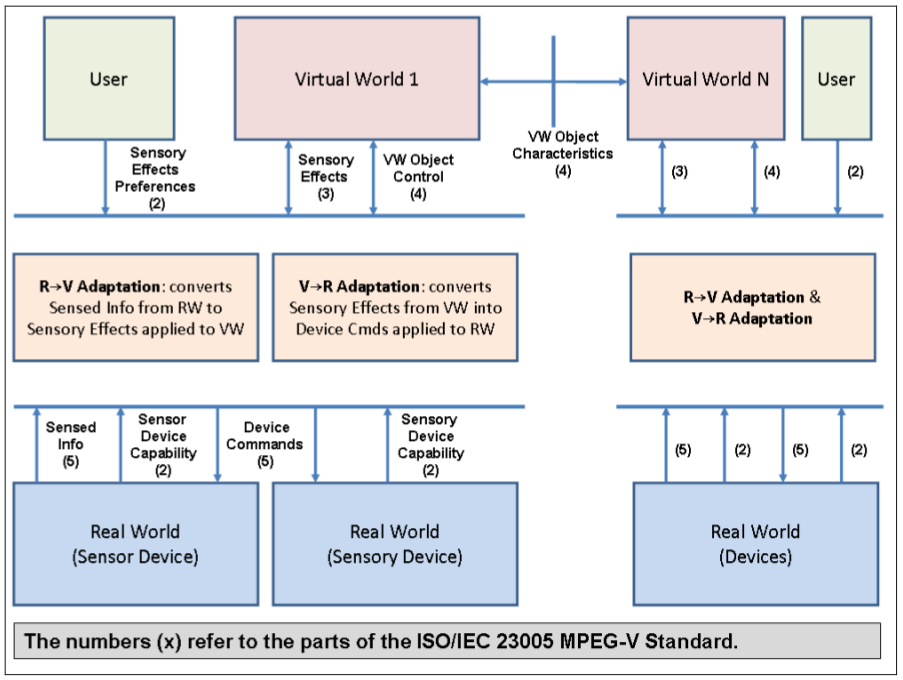
\includegraphics[width=\textwidth]{mpeg_-_v_diagram.png}
\caption{MPEG-V overview as of December 2011.}
\label{mpeg_-_v_diagram.png}
\end{figure}


\subsubsection{IEEE P1828 - Standard for Systems with Virtual Components}
Due to possible licensing issues associated with MPEG-V, with some people envisaging a similar situation as with MP3 where in September 1998 Fraunhofer IIS sent a `letter of infringement' to several small commercial and open source MP3 development projects, claiming that due to patents related to MP3 and held by Fraunhofer, all encoders (even those given away free) required the payment of royalties, a truly `open', patent-free and zero litigation alternative to MPEG-V, the IEEE Standard for Systems with Virtual Components, is under development as IEEE working group P1828~\cite{IEEE}. This endeavour is still in the concept phase, with a draft set for completion before the end of 2012. From the current draft document

\begin{quote}
\textit{``This standard is an over-arching standard for virtual environments. The over-arching standard provides a reference model and covers subsequent standards for virtual worlds. This standard establishes terminology for the Virtual Environment (VE) components and systems. The reference model covers addresses, interfaces, and/or communication protocols between and among system components. Components include supporting devices, like servers, reality engines/environments, virtual objects including avatars, and scripts. This standard defines processes, conventions and protocols to promote interoperability objects between and among virtual environments and networked resources. This standard is application agnostic but will provide illustrative use cases.''}
\end{quote}

\begin{quote}
\textit{``The purpose of this standard is to promote leverage (software and data reuse) of work between virtual project developments and promote shared resources. Another purpose of this standard is to establish the means to incorporate the respective strengths of different virtual environments. The purpose is to define a comprehensive abstraction of functions that virtual worlds can implement to interoperate at negotiable levels in near-real-time.}~\cite{InstituteofElectricalandElectronicsEngineers2012}
\end{quote}

One of the use cases already presented in the draft, under the title `Augmented and Mixed Reality'

\begin{quote}
\textit{``...covers a virtual environment with interfaces with real devices. Real devices will report status to include geolocation that would be reflected in world. Real devices will also respond to control from in-world avatars and/or scripts.''}
\end{quote}

Which clearly alludes to both virtual-to-real, augmented reality control and real-to-virtual, augmented virtuality control, supporting the standard's suitability for enabling cross reality systems and/or systems that permit simultaneous presence in real and virtual environments.
\\
\\
\\
Ultimately the realisation of cross reality and support for simultaneous presence in real and virtual environments will likely come through the development and deployment of both of these concepts; combining both an easy way to access and control sensor/actuator infrastructure via a standardized abstraction and an easy way to integrate this access and control into a virtual environment through standardized interfaces and encodings.

\section{Use Cases}
This section presents two use cases for simultaneous presence in real and virtual environments and illustrates the two different relationships that can exist between the real and virtual environments - whether they are \textit{spatially equivalent} or not.

\subsection{Virtual Time Windows - Spatial Equivalence}
\label{subsec:vtw}
The ongoing Virtual Time Window (VTW) project is an application of simultaneous presence in real and virtual environments within the domain of cultural heritage that promises to further existing alternate reality work in the field by allowing simultaneous exploration of a real cultural heritage site and its virtually reconstructed counterpart via a tablet computer~\cite{Davies2012}. A visitor to a cultural heritage site, such as the ruins of the cathedral at St Andrews, uses a tablet computer that in effect presents a `window' into a virtual reconstruction of the entire site as it was at an earlier point in time, such as the cathedral in its 13th century splendour.

To maintain a natural and unhindered sense of exploration VTW does not require visitors to manually control navigation within the virtual environment. Changes in the tablet's position within the site are automatically reflected by a corresponding movement of the avatar within the virtual environment, making use of a combination of location tracking technologies. The direction that a visitor faces is monitored by magnetometer and the angle that they hold the tablet at by accelerometer; this information is reflected by the direction and pitch of the camera within the virtual environment. The resulting style of interaction is similar to using a digital camera to take a photo; the screen on the back of the camera shows what the image will look like when the shutter is released, whilst with VTW the screen on the tablet shows what the site looked like in the past.

This approach addresses the vacancy problem by presenting the user with a convenient and natural manner in which to interact with the virtual environment whilst simultaneously exploring the real environment. A tablet computer is small, light and easy to carry and by controlling the position and direction of the camera by sensing the user's physical movements the user doesn't have to pay close attention to manually navigating within the virtual environment which would risk introducing vacancy from the real environment.

By using a complete virtual environment, rather than adding sparse virtual augmentations to a user's view of the real location in an augmented reality fashion, interactions between users at the site and those who are physically elsewhere are possible via the virtual environment.

With VTW, the virtual environment is based upon the real environment. Even though certain features may differ, for example where ruins stand in the real environment a complete building may stand in the virtual environment, there is a fundamental spatial equivalence between the two environments - they are both in effect the same `location' or `place', in an abstract sense of the terms. It is this relationship that permits the project to map a user's physical position in the real environment to an equivalent position within the virtual environment, allowing them to navigate both when in affect only controlling their navigation in one.

One might consider the `Second Earth' concept to be the ultimate realisation of this scenario of spatially equivalent real and virtual environments. Discussed by Wade Roush in a 2007 article of MIT's Technology Review magazine~\cite{Roush2007}, which is cited by Lifton in his thesis, Second Earth is theorised as the combination of the notions of virtual world technology (as in Second Life) with `mirror world' technology (as in Google Earth); Second Earth theorises a virtual simulation/reconstruction of the entire physical world, such that for any location in the real world there is a corresponding location in the virtual world. Such a resource would allow for simultaneous presence in corresponding real and virtual environments to take place anywhere, rather than being restricted to specific real world locations for which a corresponding virtual location had been created, such as a cultural heritage site.

Furthermore, if one were to apply the concepts of cross reality to such a global virtual reconstruction, it would in effect create a complete parallel virtual Earth that would react in real-time to events in the real world via sensor infrastructure and would be able to affect the real world in real-time through actuator infrastructure.

Naturally the Second Earth concept will remain just that - a concept - likely for decades, as the underlying technologies and infrastructures are not yet available to us. In a blog post on the subject of virtual world/mirror world mashups~\cite{Bar-Zeev2007}, Avi Bar-Zeev estimates that the Second Life server model at the time would require 2.4 billion physical servers to host a simulation of the entire surface of the Earth, or 1400 servers just for Manhattan. In a comment on this post, Roush emphasises that his article in Technology Review was not meant to be taken as a premise for a literal Second Life/Google Earth mashup, but that they were the leading virtual world/mirror world technologies at the time and that overlap was sure to happen.

\subsection{Snow Crash - No Spatial Equivalence}
In the opening quote to this review, taken from Neal Stephenson's cyberpunk novel \textit{Snow Crash}, the protagonist enquires about the location of another character, called Y.T., both in the real world and in the `Metaverse'. For the sake of this discussion, this Metaverse can be considered analogous to a virtual world akin to Second Life, accessed via a head mounted display, and comprises an entirely synthetic virtual world whose locations have no counterparts in the real world. Y.T.'s response is that \textit{``In  the Metaverse, I'm on a plusbound monorail train. Just passed by Port 35.''} whilst in reality she is at a \textit{``Public terminal across the street from a Reverend Wayne's"}.

In this scenario there is no spatial equivalence between the real environment and the virtual environment - they are not the same `location' or `place' as is the case with VTW - however the concept of simultaneous presence in both can still be useful, as illustrated later in the book. Y.T. is in fact waiting for a third character, Ng, to come and collect her, which leads to the following conversation in the Metaverse between Y.T. and Ng

\begin{quote}
\textit{``\ldots you're driving?''}
\\
\\
\textit{``Yes. I'm coming to pick you up - remember?''}
\\
\\
\textit{``Do you mind?''}
\\
\\
\textit{``No,'' he sighs, as if he really does.}
\\
\\
\textit{Y.T. gets up and walks around behind his desk to look.}
\\
\\
\textit{Each of the little TV monitors is showing a different view out his van; windshield,  left  window,  right  window, rearview.  Another  one  has  an electronic map  showing his position: inbound on the San Bernardino, not far
away.}
\\
\\
\textit{``The  van  is  under  voice  command,''  he  explains.  ``I  removed  the steering-wheel-and-pedal  interface because  I found  verbal  commands  more convenient. This  is why I will  sometimes  make unfamiliar  sounds with  my voice - I am controlling the vehicle's systems.''}
\end{quote}

Ng is driving his van in the real world to come and collect the real Y.T, whilst simultaneously sitting in his virtual house in the Metaverse having a conversation with the virtual Y.T., using a series of virtual TV monitors in the Metaverse to inform him of his real surroundings and to allow him to control the van.

In this scenario there is necessarily no spatial equivalence between the real environment and the virtual environment, as the virtual environment has no spatial equivalent in the real world - the monorail and Ng's house have no real counterparts. However a lack of spatial equivalence between the real environment and the virtual environment could also arise when the virtual location does have a real counterpart, but the user isn't there. For example, in reality a user could be in London whilst in the virtual environment they could be in a location that is spatially equivalent to a real part of Hong Kong.

It is already common to see people interacting with their real location, even if that interaction is limited to just walking from A to B without bumping into too many other people or being run over by a bus, whilst simultaneously interacting with the 2D Web, social media and textual chat via mobile devices such as mobile phones and tablets. With the continued trend toward the 3D Web, it is no leap to imagine a near future in which people regularly want to interact with a 3D virtual environment that is not spatially equivalent to their current location at the same time as walking to the bus stop, thus simultaneous presence in real and virtual environments that are not spatially equivalent promises to be a desirable scenario.

\section{Conclusions}
We are rapidly approaching a situation in which ubiquitous sensor/actuator infrastructure allows us to access vast amounts of information about any location at any time and additionally to act upon this information and affect these locations. The continuing adoption of fast Internet connections, the increasing ability of commodity hardware including portable devices such as mobile phones and tablets to render complex three-dimensional graphics, and the development of 3D multi-user virtual environments that place an emphasis on notions of community, creation and commerce instead of competitive gaming, all point toward a continuing natural progression toward 3D extension of the Web on a large scale.

It is already common to see people spending substantial amounts of time immersed in the 2D textual/graphical Web whilst simultaneously interacting with the real world around them. This desire to maintain a Web presence whilst simultaneously interacting with the real world is set to remain as interaction with the Web evolves from 2D to 3D. Thus it is prudent to investigate approaches for implementing and applications for exploiting the concept of simultaneous presence in real and virtual 3D environments, whether spatially equivalent or not.

This review has unearthed a plenitude of research on numerous alternate realities, either experienced in isolation from other realities (reality, virtual reality) or by mixing limited amounts of one with another (augmented reality, augmented virtuality) however has discovered a comparative lack of research attention focussed on the concept of simultaneous presence and interaction with two complete environments, one real and the other virtual. Cross reality is the closest existing concept, however the vast majority of the research in this field has used statically located computers to access the virtual environments, preventing users from exploring or interacting with the real environment that is not immediately surrounding them; the true notion of simultaneous presence in real and virtual environments requires freedom of movement and interaction with both environments, perhaps by adopting a manner of interaction with the virtual environment similar to that of the VTW project.

This deficiency of research into simultaneous presence in real and virtual environments warrants addressing with further academic investigation, as it represents a style of interaction that is bound to become commonplace as progress toward 3D extension of the Web continues at an accelerated pace.